
% Cal Poly Thesis
% 
% based on UC Thesis format
%
% modified by Mark Barry 2/07.
%

%---- SETUP SHENANIGANS ----%

\documentclass[12pt]{ucthesis}

\usepackage{float}
\usepackage{textcomp}
\usepackage{url}
\usepackage{listings}
\lstset{
    language=[Visual]C++,
    keywordstyle=\bfseries\ttfamily\color[rgb]{0,0,1},
    identifierstyle=\ttfamily,
    commentstyle=\color[rgb]{0.133,0.545,0.133},
    stringstyle=\ttfamily\color[rgb]{0.627,0.126,0.941},
    showstringspaces=false,
    basicstyle=\small,
    numberstyle=\footnotesize,
    numbers=left,
    stepnumber=1,
    numbersep=10pt,
    tabsize=2,
    breaklines=true,
    prebreak = \raisebox{0ex}[0ex][0ex]{\ensuremath{\hookleftarrow}},
    breakatwhitespace=false,
    aboveskip={1.5\baselineskip},
  columns=fixed,
  upquote=true,
  extendedchars=true
% frame=single,
% backgroundcolor=\color{lbcolor},
}
\usepackage{color}

\usepackage[pdftex]{graphicx}
\usepackage{subfig}
\usepackage{multirow}
\usepackage[chapter]{algorithm}
\usepackage{algorithmicx}
\usepackage{algpseudocode}

% Update title and author below...
\usepackage[pdftex,plainpages=false,breaklinks=true,colorlinks=true,urlcolor=blue,citecolor=blue,
linkcolor=blue,bookmarks=true,bookmarksopen=true, bookmarksopenlevel=3,pdfstartview=FitV,
   pdfauthor=Ryan Schmitt,
   pdftitle=GPU-Accelerated Point-Based Color Bleeding,
   pdfkeywords={thesis, masters, cal poly, rendering, global illumination, GPU, acceleration}
   ]{hyperref}
   %Options with pdfstartview are FitV, FitB and FitH
   \pdfcompresslevel=1

\usepackage{amssymb}
\usepackage{amsmath}
\usepackage{amsthm}
\usepackage[letterpaper]{geometry}
\usepackage[overload]{textcase}


\bibliographystyle{abbrv}

\setlength{\parindent}{0.25in} \setlength{\parskip}{6pt}

\geometry{verbose,nohead,tmargin=1.25in,bmargin=1in,lmargin=1.5in,rmargin=1.3in}

\setcounter{tocdepth}{2}


% Different font in captions (single-spaced, bold) ------------
\newcommand{\captionfonts}{\small\bf\ssp}

\makeatletter  % Allow the use of @ in command names
\long\def\@makecaption#1#2{%
  \vskip\abovecaptionskip
  \sbox\@tempboxa{{\captionfonts #1: #2}}%
  \ifdim \wd\@tempboxa >\hsize
    {\captionfonts #1: #2\par}
  \else
    \hbox to\hsize{\hfil\box\@tempboxa\hfil}%
  \fi
  \vskip\belowcaptionskip}
\makeatother   % Cancel the effect of \makeatletter
% -------------------------------------------------------------

\begin{document}

% Declarations for Front Matter

% Update fields below!
\title{GPU-Accelerated Point-Based Color Bleeding}
\author{Ryan Schmitt}
\degreemonth{December} \degreeyear{2011} \degree{Master of Science}
\defensemonth{December} \defenseyear{2011}
\numberofmembers{3} \chair{Zo\"{e} Wood, Ph.D.} \othermemberA{Chris Lupo, Ph.D.} \othermemberB{Michael Haungs, Ph.D.} \field{Computer Science} \campus{San Luis Obispo}
\copyrightyears{seven}

\maketitle

\begin{frontmatter}

% Custom made for Cal Poly (by Mark Barry, modified by Andrew Tsui).
\copyrightpage

% Custom made for Cal Poly (by Andrew Tsui).
\committeemembershippage

%---- Abstract ----
\begingroup
\begin{abstract}

Traditional Global Illumination lighting techniques like Radiosity and Monte Carlo sampling are computationally expensive. This has prompted the development of the Point-Based Color Bleeding (PBCB) algorithm by Pixar in order to approximate complex indirect illumination while meeting the demands of movie production; namely, reduced memory usage, surface shading independent run-time, and faster renders than the aforementioned lighting techniques \cite{bib:christensen2008}.

The PBCB algorithm works by discretizing a scene's directly illuminated geometry into a point cloud (surfel) representation. When computing the indirect illumination at a point, the surfels are rasterized onto cube faces surrounding that point, and the constituent pixels are combined into the final, approximate, indirect lighting value. This algorithm achieves better performance than Monte Carlo ray-tracing, but we attempt to enhance it further.

Thus, in this thesis we present a performance enhancement to the Point-Based Color Bleeding algorithm through hardware acceleration; our contribution incorporates GPU-accelerated rasterization into the cube face raster phase. The goal is to leverage the powerful rasterization capabilities of modern graphics processors in order to speed up the PBCB algorithm over standard software rasterization. Additionally, we contribute a preprocess that generates triangular surfels, uniquely suited for fast rasterization. Our algorithm reproduces the output of the traditional Monte Carlo technique, but reduces its run-time by an order of magnitude. 

\end{abstract}


\endgroup

%---- Acknowledgements ----
\begin{acknowledgements}
   Thank you...
\end{acknowledgements}


%---- Navigation ----
\tableofcontents
\listoftables
\listoffigures
\listofalgorithms


\end{frontmatter}

\pagestyle{plain}

\renewcommand{\baselinestretch}{1.66}


% ------------- Main chapters here --------------------

%---- Introduction ----
\begingroup
\chapter{Introduction}

%-------------------------------------------------------------------------------
% SECTION: Computer Graphics
%-------------------------------------------------------------------------------
\section{Computer Graphics}
Computer graphics is, in general, anything produced by a computer that isn't plain text or sound. Although, perhaps a more fitting definition is using a computer to draw a picture; this is also called rendering. There are a vast array of different areas in which one may want the help of a computer to render an image, from the entertaining, like video games and animated films, to the scientific, like medical visualization and computer-aided design and drafting. Each of these disciplines can have varying requirements of computer graphics: some need real-time rendering in order to respond to user-input, and others may trade the real-time speed for precise simulation. The goal of computer graphics is to identify the requirements of the application and render the highest quality image given those restrictions.

%-------------------------------------------------------------------------------
% SECTION: Ray-Tracing and Global Illumination
%-------------------------------------------------------------------------------
\section{Ray-Tracing and Global Illumination}
\label{sec:ray_tracing_intro}
In particular, this thesis is concerned with ray-traced rendering using Global Illumination algorithms, which are most commonly utilized to produce high-quality photo-realistic images. A ray-tracing algorithm can be classified as a Global Illumination algorithm when it incorporates not only direct illumination from light sources, but indirect illumination, or light that is inter-reflected between scene geometry from the same light sources (Figure \ref{fig:compare_illumination}).

\begin{figure}[h!]
    \centering
    \subfloat[Direct Only]{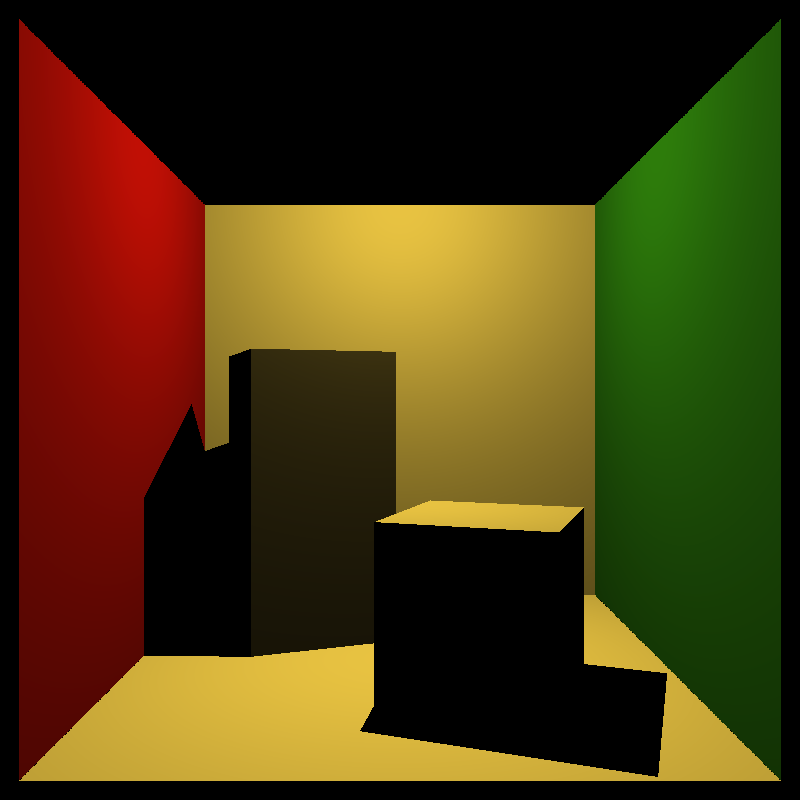
\includegraphics[width=70mm]{../img/cornell_simp_direct_only.png}}
    ~
    \subfloat[Direct \& Indirect]{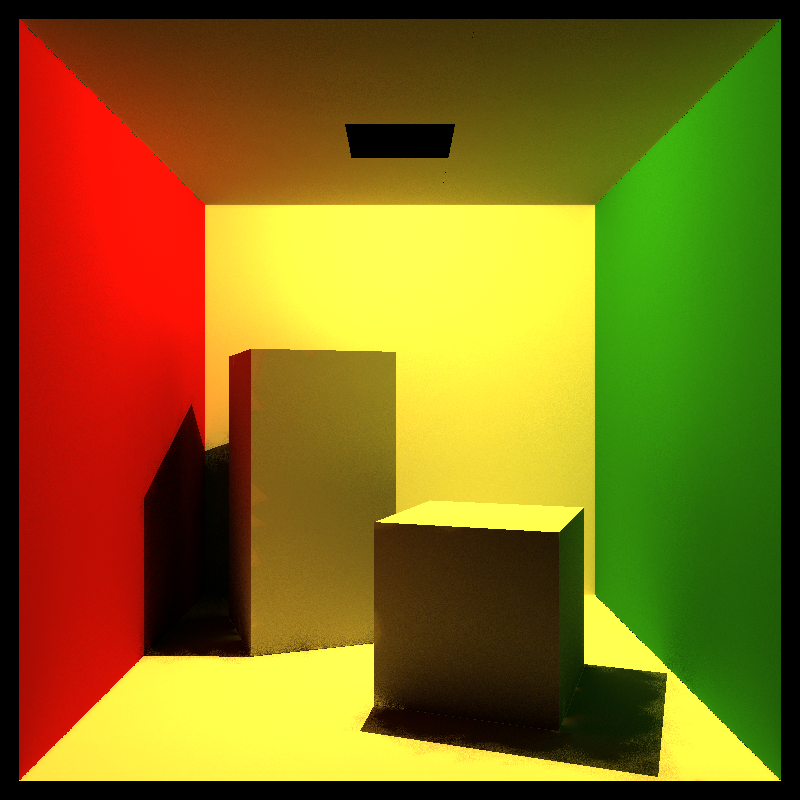
\includegraphics[width=70mm]{../img/cornell_simp_indirect.png}}
    \caption[Cornell Box direct \& indirect illumination]{Cornell Box rendered with both direct illumination and direct \& indirect illumination.}
    \label{fig:compare_illumination}
\end{figure}

Ray-tracing achieves photo-realism by simulating the physics of light using a scene comprised of light sources, mathematically-defined geometric surfaces, and a virtual camera (see figure \ref{fig:camera}). It produces renders that are specifically not real-time in nature, but meant to take as long as is necessary to produce quality results. In this setting, we must render life-like images, so an accurate simulation of light physics is required, but oftentimes we can obtain a convincing result using approximations. Specifically, ray-tracing follows the opposite path of the light: instead of tracing light rays from the light sources until they happen to hit the virtual camera, which is very physically accurate, we start at the camera and trace into the scene.

\begin{figure}[h!]
    \centering
    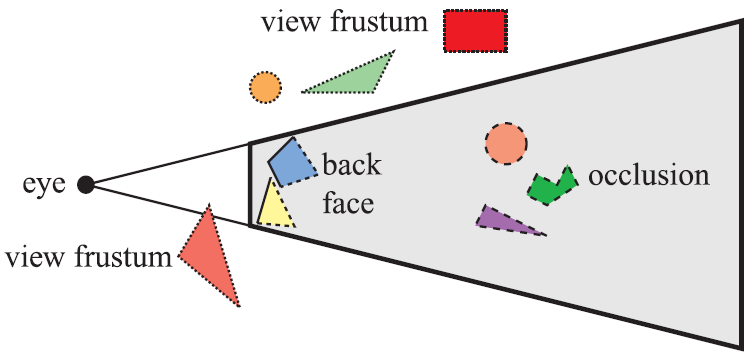
\includegraphics[width=100mm]{../img/RTR3_14_09_camera.png}
    \caption[Virtual camera, frustum, and geometry]{The eye and virtual camera are equivalent, geometry that lies in the viewing frustum is rendered. \cite{bib:rtr}}
    \label{fig:camera}
\end{figure}

Once these primary rays travel from the camera, into the scene, and intersect with the geometry, we can calculate the shading at that point in order to determine the color of the primary ray's associated pixel in the final rendered image. This shading calculation can vary from a simple direct illumination computation, to a complex Global Illumination calculation.

In this thesis, we focus on Global Illumination techniques. We split the calculation into direct illumination, which is the amount of light that leaves the source and directly intersects our shading point, and indirect illumination, which is the amount of light contributed from the diffuse inter-reflections of geometry in the scene; a phenomenon that is exemplified by the fact that the space under our desks is not completely dark, or that an illuminated red wall may reflect red light onto a nearby white box, causing it to appear reddish. These two components (direct and indirect illumination) are combined into one value that represents the incoming illumination at our primary ray's intersection point. We solve for the amount of this illumination that follows back along the ray to the camera, and we write that value to the primary ray's associated final-image-pixel. Performing this ray-tracing algorithm on each such final-image-pixel generates a rendering of the scene geometry as defined by the light sources and virtual camera, and is classified as Global Illumination.

%-------------------------------------------------------------------------------
% SECTION: Monte Carlo Ray-Tracing
%-------------------------------------------------------------------------------
\section{Monte Carlo Ray-Tracing}
\label{sec:monte_carlo}
One of the most widely used methods for the indirect illumination calculation in ray-tracing is called Monte Carlo sampling, and it involves randomly and discretely sampling the hemisphere above an intersection point (Figure \ref{fig:monte_carlo}). This is performed by recursively tracing yet more rays into the scene in order to gather information about what geometry is nearby and what color it is shaded; this attempts to solve for the diffuse inter-reflections incident at an intersection point. 

\begin{figure}[h]
   \centering
   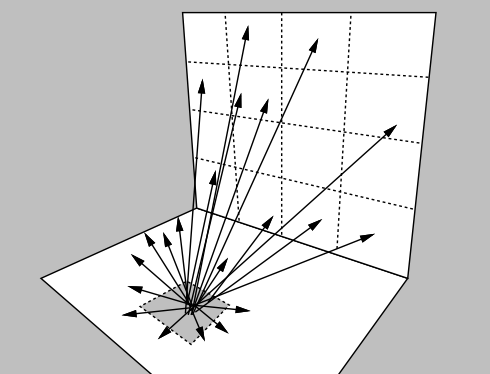
\includegraphics[width=80mm]{../img/shirley_monte_carlo.png}
   \captionfonts
   \caption[Monte Carlo hemisphere]{Monte Carlo sampling of a hemisphere above an intersection point \cite{bib:shirley1991}.}
   \label{fig:monte_carlo}
\end{figure}

Typically, around 128 of these rays are traced from each primary ray intersection point, into the scene, in order to gather enough shading information about the adjacent geometry to calculate a believable indirect illumination value. The number of rays that require intersection calculations, and shading calculations, can quickly escalate into the tens and hundreds of millions. Renders requiring multiple hours to complete are not rare.

%-------------------------------------------------------------------------------
% SECTION: Point-Based Color Bleeding
%-------------------------------------------------------------------------------
\section{Point-Based Color Bleeding}
Recently, the Point-Based Color Bleeding algorithm was developed at Pixar by Per H. Christensen \cite{bib:christensen2008} for indirect illumination. Instead of tracing rays, as in Monte Carlo ray-tracing, discretized surface elements (surfels) are rasterized onto a cube of eight-by-eight-pixel images, approximating the hemisphere used in the Monte Carlo ray-tracing (Figure \ref{fig:surfel_raster}). Once the surfels have been rasterized onto the pixels of the cube faces, the pixels are weighted and convolved into one value representing the indirect illumination at a point.

\begin{figure}[p]
   \centering
   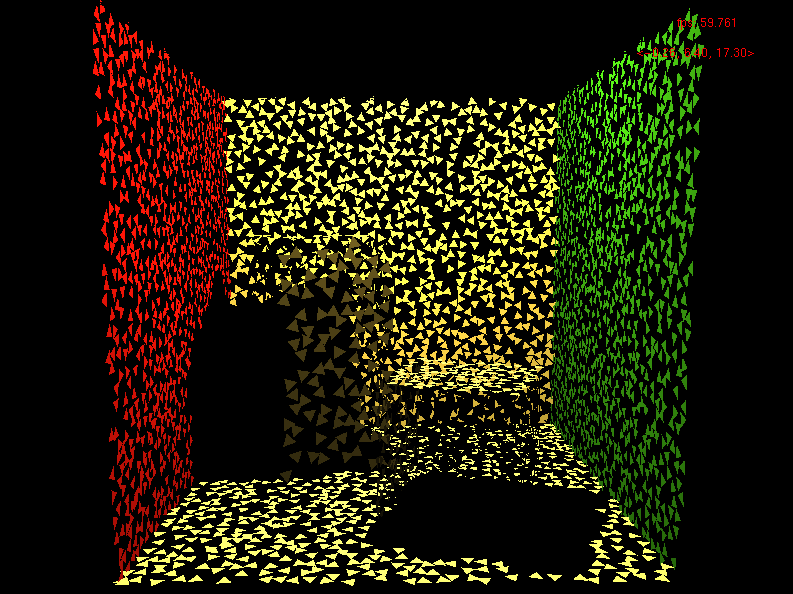
\includegraphics[width=130mm]{../img/surfel_cloud_tris.png}
   \captionfonts
   \caption[Cornell Box surfels]{Surfels for the Cornell Box scene. Note that the surfel size has been reduced to exhibit the sufel shape and distribution.}
   \label{fig:surfels}
\end{figure}

\begin{figure}[p]
   \centering
   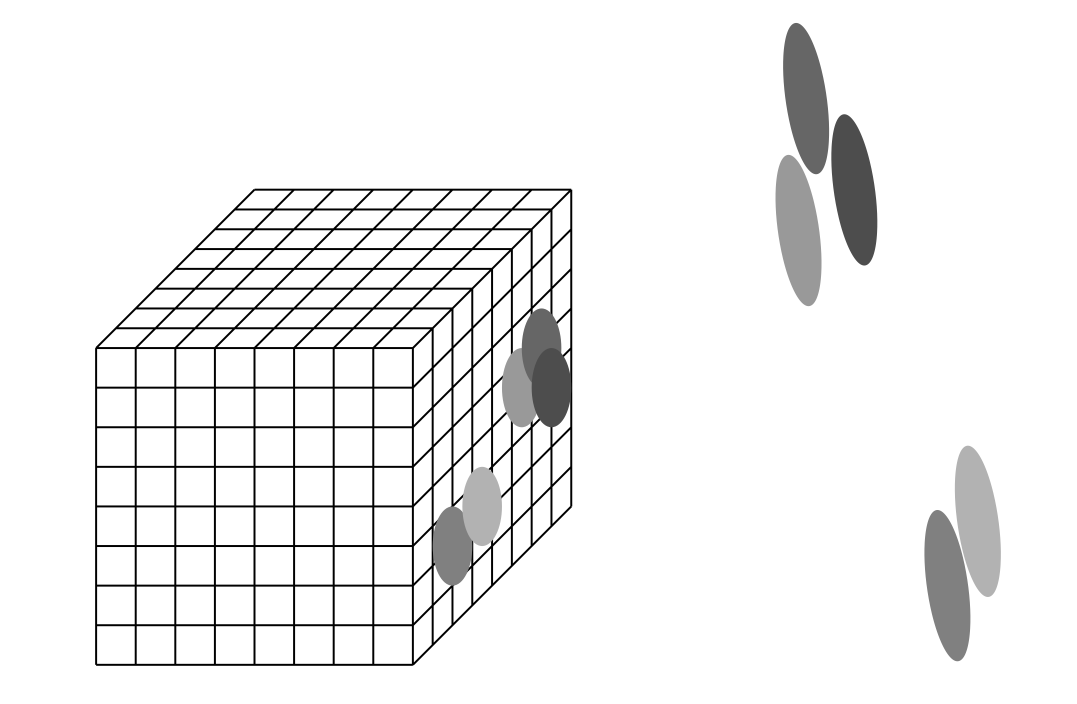
\includegraphics[width=100mm]{../img/surfel_raster.png}
   \captionfonts
   \caption[Rasterizing surfels]{Surfels being rasterized onto an 8x8 cube \cite{bib:christensen_slides}.}
   \label{fig:surfel_raster}
\end{figure}

The surfels are comprised of a location, surface normal, surface area, and shaded color computed from the direct illumination (Figure \ref{fig:surfels}). The benefit of this technique is that the surfels can be precomputed and stored in a point cloud, separate from the scene geometry, and reused. This lends itself well to reduced memory usage, surface shading independent run-time, and faster renders than Monte Carlo ray-tracing, all of which are very useful properties for Pixar and movie production in general.

%-------------------------------------------------------------------------------
% SECTION: Our Contribution
%-------------------------------------------------------------------------------
\section{Our Contribution}
This thesis is primarily concerned with performing the indirect illumination calculation faster than the Monte Carlo sampling method, without sacrificing render quality. We achieve this by extending PBCB to utilize the specialized rasterization capabilities of the modern heterogenous architecture chips' graphics processing unit (GPU) to rasterize the point cloud onto five eight-by-eight-pixel images arranged into a cube above each primary ray intersection point; this technique approximates the hemisphere that is used in the radiance integral (see section \ref{sec:radiance}). Also, we contribute a preprocess where the scene's geometry is transformed into triangles (the preferred geometric shape for GPU-rasterization) and assigned color values based on direct illumination calculations evaluated per triangle vertex.

\noindent In this paper, we:
\begin{itemize}
\item review important rendering related equations and techniques,
\item provide an in-depth description of the PBCB alrogithm,
\item present our PBCB extension and surfel generation preprocess,
\item discuss and analyze our validation techniques and results.
\end{itemize}

Our contributions, leveraging the modern heterogenous chips, realize much faster render times compared to Monte Carlo ray-tracing, while maintaining visually similar results (Figure \ref{fig:compare_techniques}). We achieve this by avoiding the numerous and costly intersection and shading calculations inherent in Monte Carlo Ray-tracing, and in some cases achieve an order of magnitude speedup.

\begin{figure}[h!]
    \centering
    \subfloat[Monte Carlo]{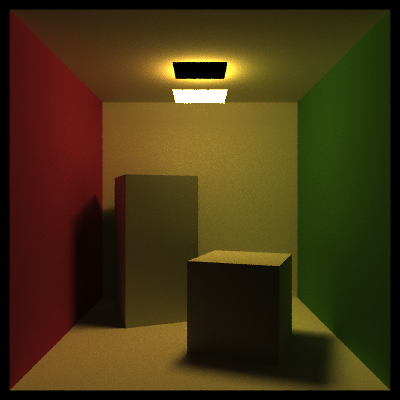
\includegraphics[width=70mm]{../img/cornell_simp_area_mcs.png}}
    ~
    \subfloat[GPU PBCB]{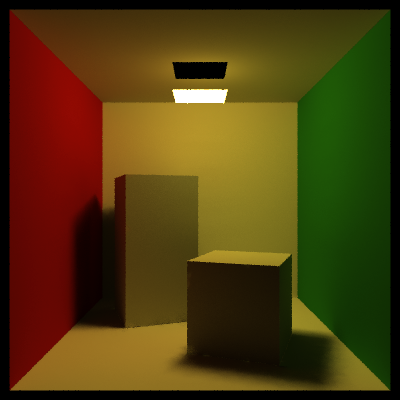
\includegraphics[width=70mm]{../img/cornell_simp_area_srf.png}}
    \caption[Cornell Box comparison]{Cornell Box with Indirect Illumination using both Monte Carlo Sampling and GPU PBCB.}
    \label{fig:compare_techniques}
\end{figure}


\endgroup

%---- Background ----
\begingroup
\chapter{Background}

%-------------------------------------------------------------------------------
% SECTION: Radiance
%-------------------------------------------------------------------------------
\section{Radiance}
\label{sec:radiance}

Radiance is a general term for the amount of light energy being transmitted through an area on a surface in a specific direction. Or more simply as the measure of brightness and color of a single ray of light \cite{bib:rtr}.

In order to understand how to calculate radiance, we must first understand radiant flux and flux density. Radiant flux, $\phi$, is a measure of energy (measured in joules) per second. Flux density is the instantaneous amount of radiant flux over an area, and is written as:
\begin{equation}
E = \frac{d\phi}{dA}
\label{eqn:flux_density}
\end{equation}
We can now define radiance as the flux density with respect to a projected area and a solid angle, or:
\begin{equation}
L = \frac{d^{2}\phi}{dA*\cos\theta*dw}
\label{eqn:radiance}
\end{equation}
Incoming radiance, or irradiance, is the radiance arriving at a surface, or the flux density of arriving light. We can define this in terms of radiance, where $x$ is a surface point and $w$ is the incoming ray direction, as:
\begin{equation}
E(x,w) = L(x,w) * \cos\theta * dw
\label{eqn:irradiance}
\end{equation}
Further more, we integrate over a hemisphere to solve for the incoming radiance, at point $x$, in all directions:
\begin{equation}
E(x) = \int L(x,w) * \cos\theta * dw
\label{eqn:irradiance_integral}
\end{equation}
Ultimately we are interested in the reflected radiance: the amount of irradiance that is reflected by a surface back towards our virtual camera. This is based on the material properties of the surface, which is typically represented by a BRDF (bi-direction reflectance distribution function). BRDFs are defined per-surface, and represented as $f(x, w^{\prime}, w)$. They solve for the ratio of radiance that is transmitted from an incoming direction, $w^{\prime}$, to an outgoing direction, $w$, at a surface point, $x$ (see figure \ref{fig:incoming_radiance}). Incorporating the BRDF, the equation for reflected radiance is:
\begin{equation}
L(p) = \int f(x, w^{\prime}, w) * L(p,w) * \cos\theta * dw
\label{eqn:radiance_integral}
\end{equation}

\begin{figure}
   \centering
   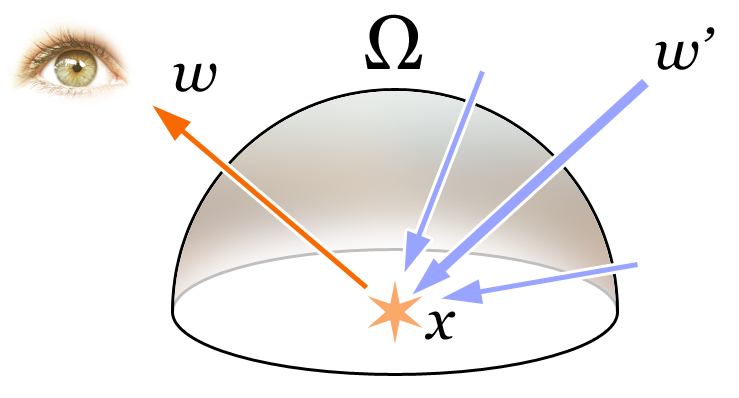
\includegraphics[width=100mm]{../img/rendering-equation-image.png}
   \captionfonts
   \caption[Incoming radiance hemisphere]{Incoming radiance in a hemisphere about a point, reflecting towards the camera. \cite{bib:nikishin_radiance}}
   \label{fig:incoming_radiance}
\end{figure}

%-------------------------------------------------------------------------------
% SECTION: Phong Reflection Model
%-------------------------------------------------------------------------------
\section{Phong Reflection Model}
\label{sec:phong_model}

The Phong reflection model is a simplified shading model used to calculate reflected radiance from one light source. It is most commonly used in scenarios that require fast computation, such as real-time graphics applications. It was presented by Phong in his University of Utah Ph.D. dissertation in 1973 \cite{bib:phong_thesis}. The equation calculates the reflected radiance using three color-vector terms: an ambient, diffuse, and specular.

The ambient component represents indirect illumination as a constant amount of reflected radiance added to all shaded points. This is the simplest term, but also poorly represents the subtleties of indirect illumination.

The diffuse component represents direct illumination using Lambertian reflectance of the incoming radiance. Lambertian refers to Lambert's cosine law, which states that, for perfectly diffuse surfaces, the diffuse reflected radiance is proportional to the cosine of the angle between the surface normal and the view vector, $\theta_{i}$. Figure \ref{fig:phong} visualizes these components.

\begin{figure}
   \centering
   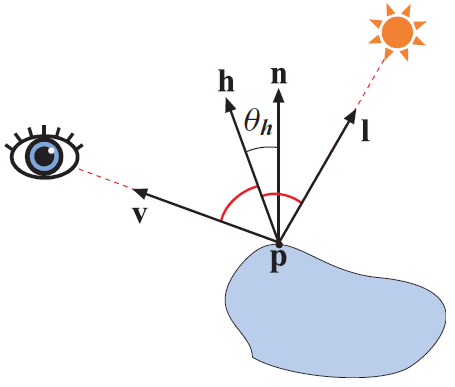
\includegraphics[width=100mm]{../img/RTR3_05_13_phong.png}
   \captionfonts
   \caption[Phong Shading Vectors]{The vectors involved in the Phong Reflectance Model. \cite{bib:rtr}}
   \label{fig:phong}
\end{figure}

The specular component represents the shininess we can view from certain angles on highly reflective surfaces. Specular reflectance is calculated by raising the cosine of the angle between the surface normal and the half vector (the vector halfway between the view and light vector), $\theta_{h}$, to the shininess of the surface, $s$.

Each of these components represent the ratio of incoming radiance, $C_{light}$ to reflected radiance, $C_{out}$, but the reflected radiance is also scaled by the surface material’s color characteristics, $C_{mat}$, as well as ambient, diffuse, and specular characteristics (represented by the scalar ratios: $M_{amb}$, $M_{diff}$, and $M_{spec}$, respectively). Combining these components we get the final Phong reflection model equation:
\begin{equation}
C_{out} = (M_{amb} * C_{mat} * C_{light}) + ((n \cdot l) * M_{diff} * C_{mat} * C_{light}) + ((n \cdot h) ^s * M_{spec} * C_{mat} * C_{light})
\label{eqn:phong}
\end{equation}

%-------------------------------------------------------------------------------
% SECTION: Anti-aliasing
%-------------------------------------------------------------------------------
\section{Anti-aliasing}
Anti-aliasing combats aliasing, the artifacting caused by under-sampling. A typical example of this in signal processing, where an analogue signal is sampled as some rate to determine it’s amplitude at that point in time. If the sample rate is too low (i.e. under-sampling) then the signal will not be accurately captured because the signal’s characteristics between samples was lost. This can be seen in Figure \ref{fig:undersampling}.

\begin{figure}[h!]
   \centering
   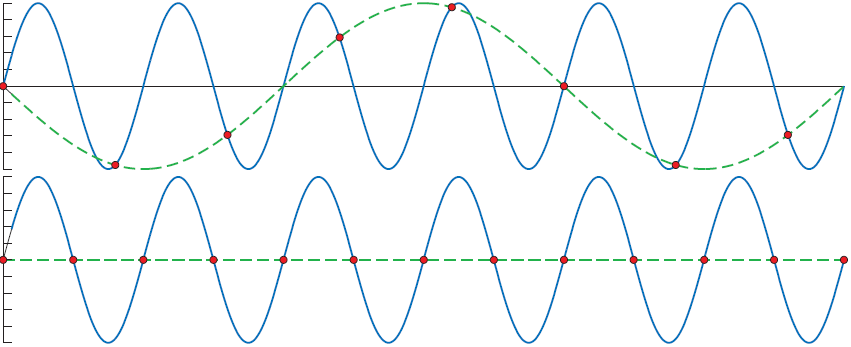
\includegraphics[width=100mm]{../img/RTR3_05_21_undersampling.png}
   \captionfonts
   \caption[Signal Undersampling]{The blue signals are being undersampled by the red dots, which leads to inaccurate reconstruction as evidenced by the dotted green line. \cite{bib:rtr}}
   \label{fig:undersampling}
\end{figure}

This occurs in computer graphics due to the limited sample rate provided by our display devices. To illustrate this point, imagine attempting to display a sphere with four pixels. More typically we experience aliasing in computer graphics as “jaggies,” or lines that should be smooth but are jagged (see Figure \ref{fig:jaggies}).

\begin{figure}[h!]
   \centering
   
\includegraphics[width=100mm]{../img/jaggies.png}
   \captionfonts
   \caption[Jaggies]{Jagged edges apparent along the silhouette edges of the top triangle are reduced via anti-aliasing techniques in the lower triangle \cite{bib:crow1977}.}
   \label{fig:jaggies}
\end{figure}

In order to combat this phenomenon, techniques for anti-aliasing have been developed. These can take many forms \cite{bib:jimenez2011}, but generally it involves some form of over-sampling (i.e. rendering the image at a multiple of the display resolution) to compensate for the fixed sample rate of our display devices. By over-sampling the rendering, we can capture the subtleties of the image in software, and can down-sample the image in a way that helps alleviate the fixed display sample rate.

The simplest form of this technique is called super-sampling: where we render an image at some multiple of the desired final resolution, and down-sample the large image back to the desired final resolution by averaging the extra pixels into one value. For example, if we wish to render a 300 by 300 pixel image, we might render an intermediate image at 600 by 600 and then each final pixel is represented by 4 intermediate pixels, which can be averaged into one final pixel value; this is called 4x super-sample anti-aliasing.

However, in order to reduce the aliasing artifacts to an acceptable level, we usually require a large super-sample rate. This can result in unacceptably long render times. The main reason we require high super-sample rates in ray-tracing is the regular pattern  created by generating rays that pass through the center of each pixel. Generally in ray-tracing, the more random you can make a sample pattern (while not missing important features), the less aliased your final image will be. Therefore, we randomly jitter the direction of each ray within the bounds of the pixel. This facilitates lower super-sample rates.

An example image of anti-aliasing in our rendering algorithm can be seen in Figure \ref{fig:anti-aliasing}.

\begin{figure}[h!]
    \centering
    \subfloat[No Anti-aliasing]{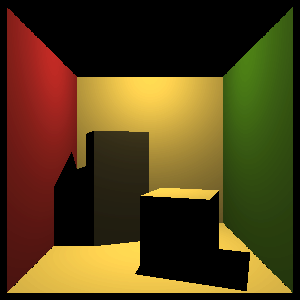
\includegraphics[width=70mm]{../img/cornell_simp_noAA.png}}
    ~
    \subfloat[9x Anti-aliasing]{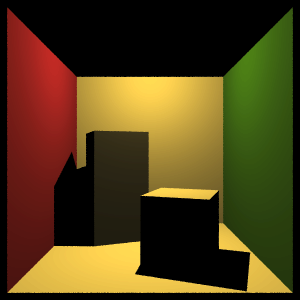
\includegraphics[width=70mm]{../img/cornell_simp_9xAA.png}}
    \caption[Anti-aliasing comparison]{Our simple Cornell box rendered with no anti-aliasing, and 9x box-filtered anti-aliasing.}
    \label{fig:anti-aliasing}
\end{figure}

%-------------------------------------------------------------------------------
% SECTION: Monte Carlo Integration
%-------------------------------------------------------------------------------
\section{Monte Carlo Integration}
\label{sec:monte_carlo_integration}

Monte Carlo integration is a technique used to evaluate integrals \cite{bib:pbr}. By repeatedly evaluating randomized discrete samples, we converge on the true evaluation of the integral. On average, these evaluations correspond to the correct solution, therefore we average multiple runs of the algorithm. We do not arrive at the correct solution in this way, but one that is statistically close.

We use Monte Carlo to evaluate the complex integral in Equation \ref{eqn:radiance_integral}. It is almost impossible to create a closed-form representation of the terms in this equation, and therefore Monte Carlo lends itself to its evaluation. To evaluate the incoming radiance at a point, we can generate randomized sample vectors (rays) over the domain of integration, the unit hemisphere. We then average these samples in order to obtain a result that is close to the true evaluation.

The main drawback of Monte Carlo integration is that it only converges at a rate of $O(n^{-1/2})$, with n being the number of discrete random samples. This means that increasing the number of samples by 4 would only reduce the error by half \cite{bib:pbr}. And because each sample requires one or more rays to be traced against the scene geometry and shaded at their intersection point, it quickly becomes cost-prohibitive to obtain low-error results. Error in this technique is exhibited by adjacent pixels that have disparity in their brightness and color, or noise.

Most of the current research in Monte Carlo for computer graphics is aimed at reducing this error through methods other than increasing the sample count \cite{bib:pbr}. One technique we use to better distribute the sample rays across the unit hemisphere is to discretize the hemisphere into a grid of sample directions with higher density in areas of higher importance, namely the top of the hemisphere where the $n \cdot l$ factor is largest, and jitter each sample direction by a random amount.

%-------------------------------------------------------------------------------
% SECTION: CPU versus GPU
%-------------------------------------------------------------------------------
\section{CPU versus GPU}
\label{sec:cpu_v_gpu}

due to their purpose. The CPU is considered a serial processor that handles general computation, which is typically thought of as instruction-driven, and involves executing unpredictable instructions on irregular data and likely includes branching. The GPU, on the other hand, is a stream processor optimized for data-driven graphics rendering of more regular data with predictable memory access. \cite{bib:rtr}

Because of their differing purposes, the CPU and GPU have traditionally been divided into two physically separate components of a computer system’s architecture connected by the PCI bus. The application running on the CPU will transmit rendering data and instructions over this bus to the GPU, which will process this input and produce a rendering. Depending on the purpose of this rendering, it can either be displayed on a monitor attached directly to the GPU, or transmitted back over the bus to the CPU for additional processing. As is common in multiprocessing systems, the two common problems we experience are load balancing and communication \cite{bib:rtr}. 

Load balancing can take place between the CPU and GPU, as well as internally within the GPU. The programmer is generally responsible for handing the load balancing between these two components, while the GPU itself leverages FIFO queues between stages to avoid stalling any part of the pipeline.

The latency and bandwidth of the bus connecting the CPU and GPU can cause communication problems as well. The theoretical maximum one-way bandwidth of the PCI Express 2.0 bus is 8.0 GB/s \cite{bib:pci_press}, while if we wanted to render 300 million triangles per second we would require a rate of 10.2 GB/s just to transfer the triangles to the GPU \cite{bib:rtr}. If we want to saturate this bandwidth, we must be constantly streaming data across the bus, however this is not always the use-scenario. Many times we wish to transmit data to the GPU, process it, and send it back to the CPU. In this case, the PCI bus can become the bottleneck as it is designed for one-way streaming of data.

%-------------------------------------------------------------------------------
% SECTION: Heterogenous Chip Architectures
%-------------------------------------------------------------------------------
\section{Heterogenous Chip Architectures}
\label{sec:heterogenous_chips}

The traditional architecture for systems with both CPU and GPUs involves the PCI bus, which connects two these two disparate components. However, recent advancements have allowed chip densities so high that both CPU and GPU can fit onto one silicon chip. These architectures, that combine CPU and GPU, are called heterogenous chips.

Intel has released both Sandy Bridge and, more recently, Ivy Bridge architectures \cite{bib:intel_press} that adhere to this ethos, and AMD has released Fusion \cite{bib:amd_press}. By combining both the CPU and GPU onto one chip, the hardware can bypass the shortcomings of the PCI bus to more quickly communicate.

In systems utilizing the traditional architecture, rendering small scenes that require final data processing on the CPU would have been cost-prohibitive due to the latency required to transfer data from CPU to GPU and back again. However, with heterogenous chip architectures, we can almost ignore this latency in our algorithms; allowing for new-found simplicity.


\endgroup

%---- Related Work ----
\begingroup
\chapter{Related Work}

In this section we discuss some of the most popular methods for computing indirect illumination. We first cover the Monte Carlo gather method, which we have implemented for comparison with our GPU PBCB method. We also discuss the basic PBCB algorithm, which we have extended to leverage the rasterization power of the GPU.

%-------------------------------------------------------------------------------
% SECTION: Monte Carlo Gather
%-------------------------------------------------------------------------------
\section{Monte Carlo Gather}
\label{sec:monte_carlo_gather}

\begin{figure}
    \centering
    \subfloat{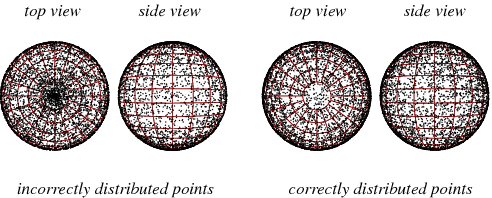
\includegraphics[width=150mm]{../img/SphericalDistribution.png}}
    \caption[Sphere Point Distribution]{Point distribution on a sphere: left is na\"{\i}ve point sampling that results in higher point density near the poles, right is correct sampling. \cite{bib:point_sampling_wa}}
    \label{fig:sphere_sampling}
\end{figure}

The Monte Carlo gather method is used in ray-tracing for indirect illumination, and receives its name from the Monte Carlo integration approximation discussed in Section \ref{sec:monte_carlo_integration}. Instead of computing the true outgoing radiance integral, which is all but impossible except in the simplest of cases, we discretize the integral and compute its approximation. We begin our description of this method at the time a ray-geometry intersection is found.

The first step is to generate the randomized sample vectors used to discretize the integral over the hemisphere. To this end, the algorithm leverages a hemisphere sampler: a function that takes two floating point variables as input, and produces a sample point on the hemisphere, see figure \ref{fig:sphere_sampling} (it should be noted that identical input always results in identical output). Typically, samplers are designed to produce a uniform random distribution over the hemisphere when two uniform random variables, $u_{1}$ and $u_{2}$, are used as input. The following equations \cite{bib:pbr} describe this mathematically:
\begin{eqnarray}
x &=& \cos (2 \pi u_{2}) \sqrt{1-u_{1}^{2}} \nonumber \\
y &=& \sin (2 \pi u_{2}) \sqrt{1-u_{1}^{2}} \nonumber \\
z &=& u_{1}
\label{eqn:uniform_hemisphere}
\end{eqnarray}

However, in some cases a uniform distribution over the hemisphere is not desired. We have found that using a purely uniform random distribution over the hemisphere does not result in acceptable noise levels until we reach approximately 256 sample vectors (see figure \ref{fig:monte_carlo_noise}).

In the case of indirect illumination computation, sample points near the top are more highly weighted then those near the bottom due to the $n \cdot l$ factor used in the Phong Shading model (see Section \ref{sec:phong_model}). Therefore, a technique called importance sampling \cite{bib:pbr} is used to create a non-uniform sampling (even though the input variables are from a uniform distribution) of the hemisphere, where the sample density increases where the $n \cdot l$ factor is largest: the top of the hemisphere. We refer to this as a cosine-weighted hemisphere sampler because the likelihood of generating a given sample point is proportional to the cosine of the angle between the vector represented by the sample point and the unit hemisphere’s vertical vector \textless$0,1,0$\textgreater. This is described mathematically in equation \ref{eqn:cosine_hemisphere} \cite{bib:pbr}.
\begin{eqnarray}
x &=& \cos (2 \pi u_{2}) \sqrt{u_{1}} \nonumber \\
y &=& \sin (2 \pi u_{2}) \sqrt{u_{1}} \nonumber \\
z &=& \sqrt{1-x^{2}-y^{2}}
\label{eqn:cosine_hemisphere}
\end{eqnarray}

An algorithm implementing equation \ref{eqn:cosine_hemisphere} is used to generate a desired number of cosine-weighted sample points on a unit hemisphere. These sample points are treated as vectors to describe the direction of sample rays used to gather incoming radiance information. In order to convert from a vector in unit hemisphere coordinates to a vector in world space coordinates we use Algorithm \ref{alg:unit_world_xform}. This is a standard coordinate system transformation between surface, or object, space and world space.

\begin{algorithm}[H]
\captionfont
\caption[Unit to World Hemisphere]{Transform from unit hemisphere to world space.}
\label{alg:unit_world_xform}
{\fontsize{10}{9}\selectfont
\begin{algorithmic}
   \Function{HemisphereTransform}{$surfaceNormal$}
      \If{$|surfaceNormal.y| = 1$}
         \State $tangent$ :=  $\textless1,0,0\textgreater$
      \Else
         \State $k := \textless0,1,0\textgreater$
         \State $tangent$ :=  $k - ((k \cdot surfaceNormal)*surfaceNormal)$ //Gram-Schmidt Process
         \State normalize($tangent$)
      \EndIf
      \State $binormal := surfaceNormal \times tangent$
      \State $transform := \bigl( \begin{smallmatrix} tangent.x & surfaceNormal.x & binormal.x \\ tangent.y & surfaceNormal.y & binormal.y \\ tangent.z & surfaceNormal.z & binormal.z \end{smallmatrix} \bigr)$
      \State \Return $transform$
   \EndFunction
\end{algorithmic}
}
\end{algorithm}

The next step is to use these transformed vectors as ray directions to perform a recursive ray tracing computation. Each computation returns the incoming radiance, just as the primary rays return incoming radiance written to a final image pixel. These incoming radiance values are convolved into one indirect illumination value for the point we are attempting to shade by computing their arithmetic mean. This results in an indirect illumination value used in the current shading computation.

Typically, the shading computations returned by the rays generated by the Monte Carlo method use direct illumination only, but because light can reflect off multiple surfaces in reality, multi-bounce Monte Carlo gather can be performed as well, to increase realism. This is where the Monte Carlo method is used recursively to calculate the indirect illumination contribution to the incoming radiance along one of the Monte Carlo sample rays. However, this is incredibly computationally expensive, and not used in this thesis.

Lastly, it is important to note that the number of samples used directly affects the presence of noise in the final image. Figure \ref{fig:256mcs} illustrates how noise levels are reduced by increasing the number of Monte Carlo samples.

%-------------------------------------------------------------------------------
% SECTION: Point Based Color Bleeding
%-------------------------------------------------------------------------------
\section{Point Based Color Bleeding}

Point Based Color Bleeding is a technique for indirect illumination computation developed by Per H. Christensen at Pixar. It specifically addresses concerns relevant to movie production, namely: surface shading independent runtime, reduced memory usage, and faster runtimes than Monte Carlo gather \cite{bib:christensen2008}. It leverages rasterization instead of ray-tracing to compute the indirect illumination component of a shading computation.

The PBCB algorithm approximates the radiance integral by gathering incoming radiance samples as rasterized cube-face pixels. When computing the indirect illumination at an intersection point, the hemisphere is approximated by a 5-faced cube, called a cube-map, where each face is an 8-by-8 pixel texture (see figure \ref{fig:surfel_raster}). The primitives that are rasterized are called surfels (surface elements) and are generated as a preprocess.

Surfels are required due to the limitations and requirements of the rasterization step: rasterization cannot support complex geometry common in ray-tracing (e.g. non-planar surfaces, like spheres, or NURBS \cite{bib:nurbs}), and in order to make it as fast as possible, it should not perform any complex shading. Each surfel is composed of a location, surface normal, radius, and color, and can be conceptualized as a disk (see figure \ref{fig:disk_surfels}). In order to adequately capture the shading information with one color per surfel, the geometry is point-sampled at a desired density and a surfel is constructed per sample point. (As an aside: we should mention that \cite{bib:christensen2008} does not describe a point-sampling algorithm, and we have developed our own as described in Section \ref{sec:point_gen}) The surfel’s location is defined by the sample point, its normal is defined by the source-geometry’s surface normal at the sample point, its radius is defined such that there are no gaps between surfels, and its color is computed by shading the sample point using only direct illumination. In this way, a direct-shaded surfel cloud representation of a scene’s geometry is generated, as in Figure \ref{fig:surfels}, and can be stored for use in rasterization.

\begin{figure}
    \centering
    \subfloat{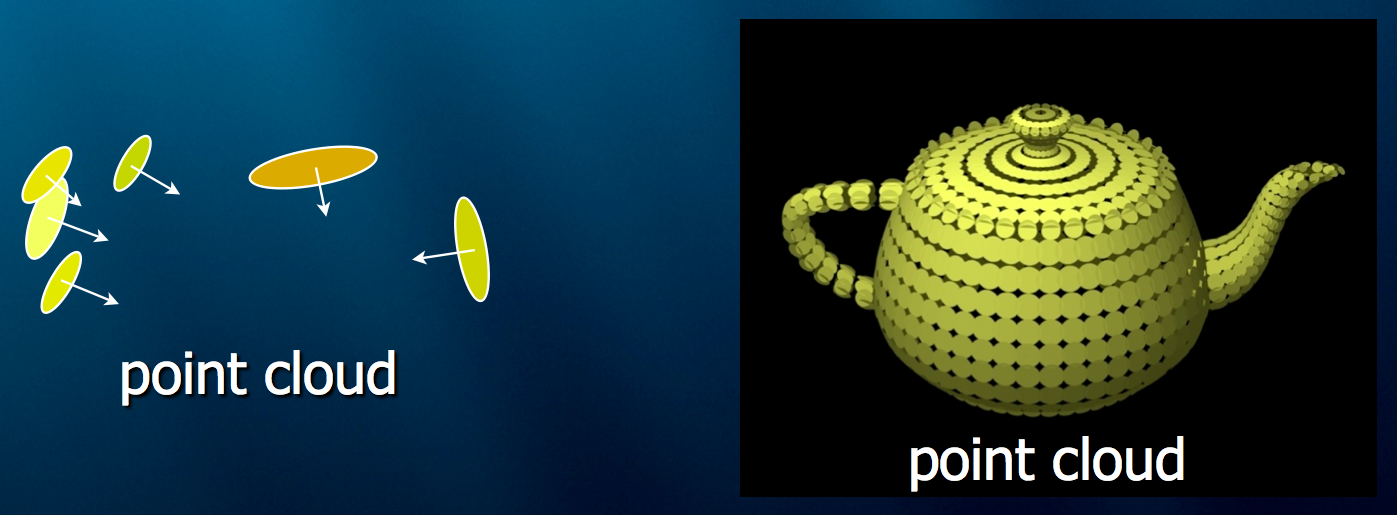
\includegraphics[width=150mm]{../img/surfel_disks.png}}
    \caption[Surfel Disks]{Surfels as disks, from Per H. Christensen's slides on the subject. \cite{bib:christensen_slides}}
    \label{fig:disk_surfels}
\end{figure}

During the course of the standard ray-tracing algorithm, the PBCB technique is used to compute the indirect illumination component required to shade an intersection point. For one point, a 5-faced cube-map is constructed such that each face is composed of an 8-by-8 pixel texture. This approximates the hemisphere used in the Monte Carlo gather technique (see figure \ref{fig:monte_carlo}).The surfel cloud is then rasterized onto the cube-map using a proprietary rasterization algorithm \cite{bib:christensen2008}. Figure \ref{fig:surfel_raster} illustrates the result.

With the surfel cloud rasterized onto the cube-map, each pixel represents the incoming radiance from its direction. The center of the pixel can be interpreted as if it were a sample point on the unit-hemisphere and the pixel’s color can be weighted using the $n \cdot l$ factor to compute the incoming radiance value from that angle. These incoming radiance values are scaled by the surface color (see section \ref{sec:phong_model}) and averaged to compute the final indirect illumination contribution to the shading computation for an intersection point.


\endgroup

%---- Algorithm ----
\begingroup
\chapter{GPU Point Based Color Bleeding}

%-------------------------------------------------------------------------------
% SECTION: Algorithm Introduction
%-------------------------------------------------------------------------------
\section{Algorithm Introduction}

Indirect Illumination presents a computationally expensive problem. Potentially, the entirety of a scene's geometry could contribute illumination to any given point for which we try to compute indirect lighting. For Monte Carlo ray-tracing, intelligent randomness, spacial data structures, and attention to writing performant code can help alleviate the problem, but we can do better.

Our algorithm uses rasterization, rather than ray-tracing, to determine the radiance during the indirect shading computation. Rasterization has traditionally been used in real-time graphics due its high throughput, but we can leverage that same throughput to reduce our time spent caculating indirect illumination. However, we want to also gain hardware acceleration, and GPU rasterization algorithms require specific input, namely triangles. Thus, we preprocess our scene geometry to convert it into a triangle-based surfel cloud, and store it in GPU memory. At render time, we can leverage the GPU to quickly rasterize these surfels, in parallel, onto cube-maps to capture the radiance at a point.

In this way, each cube-map pixel represents the radiance at the location of the cube-map, in the direction of that pixel. This is analogous to the way Monte Carlo ray-tracing casts a ray and calculates shading at its scene intersection to represent radiance, in the ray's direction, at the ray's origin.

In this chapter, we further discuss our GPU Point-Based Color Bleeding algorithm: section \ref{sec:surfel_generation} explains our preprocess for generating triangle-based surfels, section \ref{sec:rendering} follows with an explanation of our rendering pipeline. By combining our indirect illumination algorithm with GPU-hardware specifically designed for fast and parallel rasterization, we achieve quantitatively similar results in less time than Monte Carlo ray-tracing.

As an overview, the algorithm steps are as follows:

\begin{algorithm}[H]
\captionfont
\caption[GPU PBCB Algorithm]{Psuedocode for our GPU Point-Based Color Bleeding algorithm.}
\label{alg:gpu_pbcb}
{\fontsize{10}{9}\selectfont
\begin{algorithmic}
   \Function{GPUPointBasedColorBleeding}{$scene$}
      \ForAll{$geomPrimitive$ \textbf{in} $scene$}
         \State $surfels$ += GenerateSurfels($geomPrimitive$, 500) //see alg. \ref{alg:surfel_gen}
      \EndFor
      \State $rays$ := GenerateRays($scene$.imageDescription)
      \ForAll{$ray$ \textbf{in} $rays$}
         \State $intersection$ := Intersect($ray, scene$)
         \State $direct$ := DirectIllumination($intersection, scene$)
         \State $indirect$ := IndirectIllumination($intersection, scene$)
         \State $finalColor$ := $direct$ + $indirect$
         \State $image$.writeToPixel($ray$.index, $finalColor$)
      \EndFor
      \State WriteToDisk($image$)
   \EndFunction
\end{algorithmic}
}
\end{algorithm}

%-------------------------------------------------------------------------------
% SECTION: Surfel Generation
%-------------------------------------------------------------------------------
\section{Surfel Generation}
\label{sec:surfel_generation}

The PBCB algorithm relies on the abstract representation of a scene's geometry as surfels in order to leverage the power of rasterization. Real-time graphics applications also utilize rasterization, but do not use surfel representations. This is because they target specific framerates between 30 and 60 frames per second, allowing 16 to 33 milliseconds for the computation of dynamic shadows, Phong shading, texture mapping, bump mapping, and other techniques on a per pixel basis. In the case of PBCB, rasterization must perform as fast as possible. To achieve this, additional computations of the kind referred to earlier (e.g. dynamic shadows) are avoided, and the rasterization algorithm simply uses the color of the surfel directly as the pixel's color. This is the reason why the PBCB algorithm does not simply rasterize the geometric primitives as a whole, but subdivides them into surfels with one color, computed as the direct illumination at the surfel's location on the scene geometry. If this were not the case, each geometric primitive would only be represented by one color, resulting in inaccurate indirect illumination.

In the traditional PBCB algorithm, surfels are disks, but our GPU PBCB cannot use this representation. The GPU is specifically designed to render images quickly by parallelizing the work, thus increasing throughput. However, we gain this performance at the cost of generality: the GPU can only process triangles as input data. Therefore, we must translate the representation of our geometric primitives into triangles (see Figure \ref{fig:surfelcloud}).

\begin{figure}[h!]
   \centering
   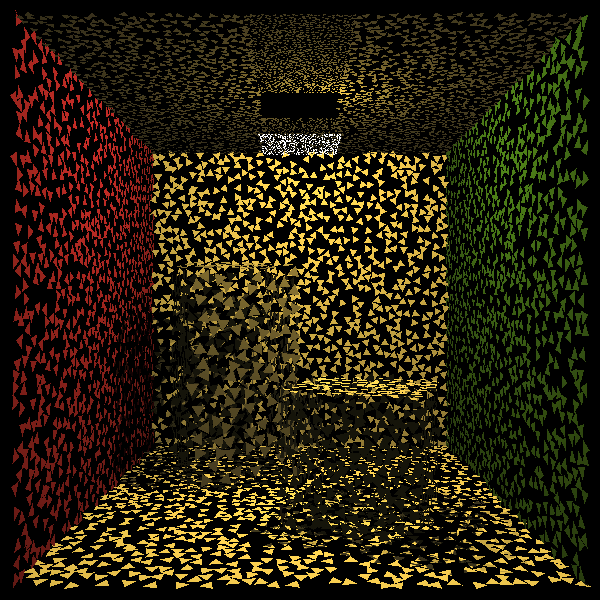
\includegraphics[width=100mm]{../img/cornell_simp_area_surfelcloud.png}
   \captionfonts
   \caption[Cornell Box with area light surfels]{The surfels generated for our Cornell Box with area light. Note that the surfel size has been reduced to exhibit the sufel shape and distribution.}
   \label{fig:surfelcloud}
\end{figure}

Each geometric primitive uses the same general algorithm to generate surfels, with differences in how the initial points are generated. We begin by generating a random distribution of points on the surface of the primitive, and use those points as the center for each triangular surfel. There has yet to be developed any algorithm with which to generate a uniformly random distribution of points on arbitrarily transformed geometry in linear time. In fact, Paul Bourke's methods in \cite{bib:bourke_spheregen} and \cite{bib:bourke_pointdist} require specific geometry that has not been transformed to generate a point distribution, and operate in polynomial time.

Our distribution algorithm is novel in its support for arbitrarily transformed geometry, but still requires polynomial time. However, because surfels are generated as a pre-process; the runtime does not affect our results. In general, we calculate our point distributions by first generating random points on the surface of our geometry, then pruning the two closest points repeatedly until we achieve the desired number of points. While in theory this algorithm does not achieve a mathematically uniform distribution, in practice it distributes the points well enough to achieve our goal of quantitatively similar results to Monte Carlo ray-tracing, is simple to understand and implement, and meets our requirement of supporting arbitrarily transformed geometry.

Once the points have been computed, the three triangle vertices are generated by adding the point's surface tangent vector to the point to solve for the first vertex, then rotating that vector by 120 degrees to solve for the second, and once more for the third. The length of the vector is determined by multiplying the distance between the two closest points and a constant. The goal is to have coverage over the surface of the geometry without superfluous gaps or overlaps. We have found that doubling the distance results in satisfactory coverage.

We discuss the general surfel generation algorithm in Section \ref{sec:surfel_gen}. We also discuss the specific point generation algorithms for boxes, spheres, and triangles in Section \ref{sec:point_gen}. In Section \ref{sec:surfel_gen} we discuss our algorithm for constructing traingular surfels, and in Section \ref{sec:VBOStorage} we discuss our storage method for these surfels.

% ---- SUBSECTION: Point Generation ----
\subsection{Point Generation}
\label{sec:point_gen}

In order to generate surfels for a any of our geometric primitives, we first generate a point distribution to act as center points for our surfels. The strategy we use for point distribution is stratified stochastic sampling.

% ---- SUBSUBSECTION: Box ----
\subsubsection{Box}
\label{sec:box_point_gen}
Points for the box primitive are generated per side. Each side is divided into a u-v grid, with a point for each intersection. We jitter the points to add randomness, which helps during the culling process explained later in this section, and to help mask any artifacting that can result from regular patterns. The pseudocode can be seen in Algorithm \ref{alg:box_point_gen}. Point distributions for a box can be seen in Figure \ref{fig:small_box_surfels}.

\begin{algorithm}
\captionfont
\caption[Box point generation]{Generate stratefied stochastic sample points for a box.}
\label{alg:box_point_gen}
{\fontsize{10}{9}\selectfont
\begin{algorithmic}
   \Function{SampleGeometry}{$box, numSamples$}
      \State $pointsPerSide := numSamples / 6$
      \State $pointsPerDim$ := sqrt($pointsPerSide$)
      \For{\textbf{each} $side$ \textbf{in} $boxSides$}
         \For{$u := 0...pointsPerDim$}
            \For{$v := 0...pointsPerDim$}
               \State $\alpha := (u + $rand($0,1$)$) / pointsPerDim$
               \State $\beta := (v + $rand($0,1$)$) / pointsPerDim$
               \If{$side$ = small z-plane}
                  \State $x := (1-\alpha) * box.start.x + \alpha * box.end.x$
                  \State $y := (1-\beta) * box.start.y + \beta * box.end.y$
                  \State $z := box.start.z$
               \ElsIf{$side$ = large z-plane}
                  \State $x := (1-\alpha) * box.start.x + \alpha * box.end.x$
                  \State $y := (1-\beta) * box.start.y + \beta * box.end.y$
                  \State $z := box.end.z$
               \ElsIf{$side$ = small x-plane}
                  \State $x := box.start.x$
                  \State $y := (1-\alpha) * box.start.y + \alpha * box.end.y$
                  \State $z := (1-\beta) * box.start.z + \beta * box.end.z$
               \ElsIf{$side$ = large x-plane}
                  \State $x := box.end.x$
                  \State $y := (1-\alpha) * box.start.y + \alpha * box.end.y$
                  \State $z := (1-\beta) * box.start.z + \beta * box.end.z$
               \ElsIf{$side$ = small y-plane}
                  \State $x := (1-\alpha) * box.start.y + \alpha * box.end.y$
                  \State $y := box.start.y$
                  \State $z := (1-\beta) * box.start.z + \beta * box.end.z$
               \ElsIf{$side$ = large y-plane}
                  \State $x := (1-\alpha) * box.start.y + \alpha * box.end.y$
                  \State $y := box.end.y$
                  \State $z := (1-\beta) * box.start.z + \beta * box.end.z$
               \EndIf
               \State $point := box.modelTransform *$ \textless$x, y, z$\textgreater
               \State $points$ += $point$
            \EndFor
         \EndFor
      \EndFor
      \State \Return $points$
   \EndFunction
\end{algorithmic}
}
\end{algorithm}

% ---- SUBSUBSECTION: Sphere ----
\subsubsection{Sphere}
\label{sec:sphere_point_gen}
Point generation for a sphere is based on a uniform sampling algorithm \cite{bib:pbr} that requires two uniform random variables as input. Instead of using entirely uniform random variables, u and v, we step through u and v coordinates, which effective subdivides the sphere into a grid. Again we jitter the coordinates to help randomize our surfel cloud.
The psuedocode can be seen in Algorithm \ref{alg:sphere_point_gen}.
Point distributions for a sphere can be seen in Figure \ref{fig:small_sphere_surfels}.

\begin{algorithm}[H]
\captionfont
\caption[Sphere point generation]{Generate stratefied stochastic sample points for a sphere.}
\label{alg:sphere_point_gen}
{\fontsize{10}{9}\selectfont
\begin{algorithmic}
   \Function{SampleGeometry}{$sphere, numSamples$}
      \State $numPointsU$ := sqrt($numSamples$)
      \State $numPointsV$ := $numSamples / numPointsU$
      \For{$i := 0...numPointsU$}
         \For{$j := 0...numPointsV$}
            \State $u := (i + $rand($0,1$)$) / numPointsU$
            \State $v := (j + $rand($0,1$)$) / numPointsV$
            \State $z := 1 - 2*u$
            \State $r$ := sqrt(max($0, 1- z*z$))
            \State $\phi := 2 * \pi * v$
            \State $x := r *$ cos($\phi$)
            \State $y := r *$ sin($\phi$)
            \State $point := \textless x, y, z \textgreater * sphere.radius + sphere.center$
            \State $point := sphere.modelTransform * point$
            \State $points$ += $point$
         \EndFor
      \EndFor
      \State \Return $points$
   \EndFunction
\end{algorithmic}
}
\end{algorithm}

% ---- SUBSUBSECTION: Triangle ----
\subsubsection{Triangle}
\label{sec:triangle_point_gen}
We generate our triangle sample points by modifying a uniform sample pattern algorithm \cite{bib:pbr} in a similar manner to our sphere point generation.
The original algorithm requires two uniformly random variables as input, and will generate a uniformly distributed random point on the triangle.
By discretizing the u and v values and stepping through them, we effectively walk a uniformly distributed grid across the triangle's surface area.
Again, we jitter the sample point location in order to eliminate any regular patterns.
The psuedocode can be seen in Algorithm \ref{alg:triangle_point_gen}.
Point distributions for a triangle can be seen in Figure \ref{fig:small_triangle_surfels}.

\begin{algorithm}[H]
\captionfont
\caption[Triangle point generation]{Generate stratefied stochastic sample points for a triangle.}
\label{alg:triangle_point_gen}
{\fontsize{10}{9}\selectfont
\begin{algorithmic}
   \Function{SampleGeometry}{$triangle, numSamples$}
      \State $numPointsU$ := sqrt($numSamples$)
      \State $numPointsV$ := $numSamples / numPointsU$
      \State $v_{0..1} := triangle.vertex1 - triangle.vertex0$
      \State $v_{0..2} := triangle.vertex2 - triangle.vertex0$
      \For{$i := 0...numPointsU$}
         \For{$j := 0...numPointsV$}
            \State $u := (i + $rand($0,1$)$) / numPointsU$
            \State $v := (j + $rand($0,1$)$) / numPointsV$
            \State // Inside or outside the triangle?
            \If{$u + v < 1$}
               \State $point := triangle.vertex0 + u*v_{0..1} + v*v_{0..2}$
            \Else
               \State $point := triangle.vertex0 + (1-u)*v_{0..1} + (1-v)*v_{0..2}$
            \EndIf
            \State $point := triangle.modelTransform * point$
            \State $points$ += $point$
         \EndFor
      \EndFor
      \State \Return $points$
   \EndFunction
\end{algorithmic}
}
\end{algorithm}

With the previous point distribution algorithms, we must address the issue of non-uniform scaling. For example, if we are generating points for a box scaled more in the y-axis than the x- or z-axis, then our computed sample points will be further spaced apart along that axis. This leaves us with a sampling pattern that is not uniform, but stretched in one direction.

Our solution to this problem is simple, easy to implement, and novel in the fact that it is geometry and transformation independent. We generate a multiple of the requested number of sample points, jitter their location, and repeatedly cull the two closest points until we arrive at the desired number of points. In this way, we work backwards to a more uniform distribution in a way that supports arbitrary geometric topology and transformations. Figures \ref{fig:small_box_surfels}, \ref{fig:small_sphere_surfels}, and \ref{fig:small_triangle_surfels} show the result of this process for varying multiples of the requested number of surfels; notice the coverage issues caused by not generating more than the requested number of surfels (e.g. Figure \ref{fig:box500s}).

The pseudocode is listed in Algorithm \ref{alg:point_gen}.

\begin{algorithm}
\captionfont
\caption[Create Points and Cull]{Create points and repeatedly cull one of the two closest points.}
\label{alg:point_gen}
{\fontsize{10}{9}\selectfont
\begin{algorithmic}
   \Function{GeneratePoints}{$geomPrimitive, numberOfSamples$}
      \State $points :=$ SampleGeometry($geomPrimitive$, $2*numberOfSamples$) //alg. \ref{alg:box_point_gen}, \ref{alg:sphere_point_gen}, \ref{alg:triangle_point_gen}
      \While{$points$.length $>$ $desiredNumPoints$}
         \State $minPointIndex :=$ FindAndRemoveClosestPoints($points$)
         \State $points$.remove($minPointIndex$)
      \EndWhile
      \State \Return $points$
   \EndFunction
\end{algorithmic}
}
\end{algorithm}

% ---- SUBSECTION: Surfel Generation ----
\subsection{Surfel Generation}
\label{sec:surfel_gen}

With the points generated, our surfel generation algorithm is quite simple: it consists of using the sample points as the center for triangular surfels. The question we must answer is what surface area will achieve adequate coverage of the source geometry. Too large of a surface area results in extending our surfel borders beyond the edges of our geometry as well as excessive surfel overlapping. Too small of a surface area results in gaps between surfels. Both of these issues will cause artifacts in our rendering by misrepresenting the source geometry.

Our algorithm uses the distance between the two closest sample points as the theoretical radius required for disk surfels to adequately cover the geometry. (In practice, we double this radius in order to ensure coverage.) In order for our triangle surfels to match this surface area, we extrapolate the length of the vector from triangle surfel center to equilateral vertex using Equation \ref{eqn:tri_dist}.

\begin{equation}
vectorLength = \sqrt{ \frac{ \pi * radius^2 }{ \sqrt{3} * \sin^2(60) } }
\label{eqn:tri_dist}
\end{equation}
~

However, the random jittering of sample points often results in initial sample points that are very close together. While the jittering produces the desired randomness, it also gives us too low an estimate of the required radius; the result of which can be seen in Figure \ref{fig:box500}. But the aforementioned point culling solution (see Section \ref{sec:point_gen}) also solves this problem. By culling the closest points, we create a more uniform distribution with less variance in the distance between adjacent sample points.

For typical surfel generation times per geometric primitive, see Table \ref{tbl:surf_gen_times}. In psuedocode, our surfel generation algorithm is listed in Algorithm \ref{alg:surfel_gen}. And Figure \ref{fig:surfel_cloud_simple} is a rendering of the raw surfel cloud in OpenGL without any lighting.

\begin{figure}
   \centering
   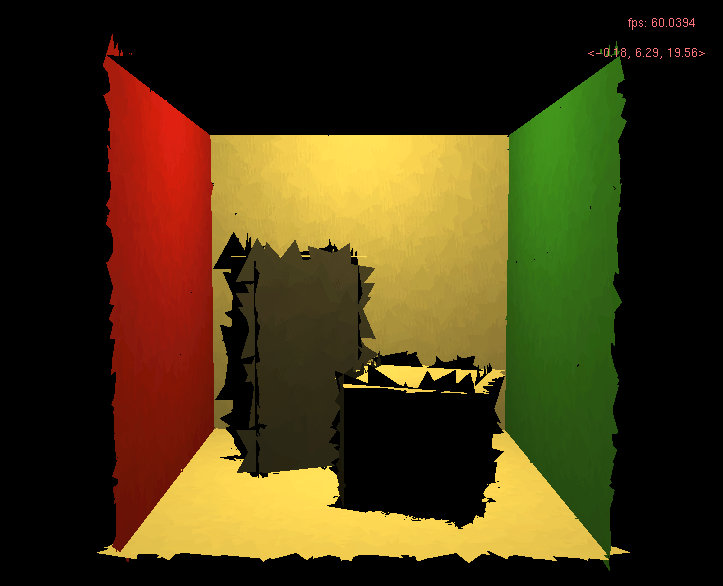
\includegraphics[width=100mm]{../img/surfel_cloud_simple.png}
   \captionfonts
   \caption[OpenGL Cornell Box surfel cloud]{Surfels generated for the Cornell Box scene rendered, without lighting, in OpenGL using a VBO.}
   \label{fig:surfel_cloud_simple}
\end{figure}

\begin{algorithm}[H]
\captionfont
\caption[Surfel generation]{Generate surfels from points on a geometric primitive.}
\label{alg:surfel_gen}
{\fontsize{10}{9}\selectfont
\begin{algorithmic}
   \Function{GenerateSurfels}{$geomPrimitive, numberOfSurfels$}
      \State $points :=$ GeneratePoints($geomPrimitive, numberOfSurfels$) //see alg. \ref{alg:point_gen}
      \State $minD :=$ FindClosestPoints($points$)
      \State $vectorLength := 2 * $sqrt(($PI * minD * minD$)$ / 1.299$) //see eqn. \ref{eqn:tri_dist}
      \ForAll{$point$ \textbf{in} $points$}
         \State $tangent :=$ CalculateTangent($point, geomPrimitive$)
         \State $surfel :=$ new surfel
         \State $surfel.v0 := point + vectorLength * tangent$
         \State $surfel.v1 := point + vectorLength * $rotate($tangent, 120$)
         \State $surfel.v2 := point + vectorLength * $rotate($tangent, 240$)
         \State $surfels$.add($surfel$)
      \EndFor
      \State \Return $surfels$
   \EndFunction
\end{algorithmic}
}
\end{algorithm}

\vfill
\begin{table}[h!]
   \centering
   \begin{tabular}{ | l | l | l | l | l | l | }
   \hline
   & \textbf{500 pts.} & \textbf{1000 pts.} & \textbf{2000 pts.} & \textbf{4000 pts.} & \textbf{8000 pts.} \\ \hline
   \textbf{Box} & 1ms & 430ms & 5s 927ms & 43s 104ms & 6m 24s 819ms \\ \hline
   \textbf{Sphere} & 1ms & 714ms & 6s 274ms & 51s 286ms & 6m 50s 309ms \\ \hline
   \textbf{Triangle} & 1ms & 713ms & 6s 341ms & 51s 279ms & 6m 49s 847ms \\ \hline
   \end{tabular}
   \captionfonts
   \caption[Surfel generation times]{Surfel generation times listed by geometric primitive versus number of initial points.}
   \label{tbl:surf_gen_times}
\end{table}
\vfill
                        
\begin{figure}[h!]
   \centering
   \subfloat[500 points (1ms)]{\label{fig:box500s}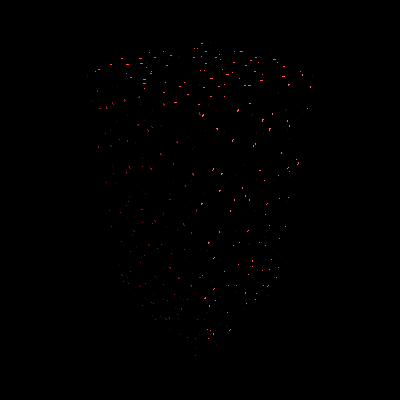
\includegraphics[width=50mm]{../img/box_500_initial_points_quarter_size_1ms.png}}
   ~
   \subfloat[1000 points (430ms)]{\label{fig:box1000s}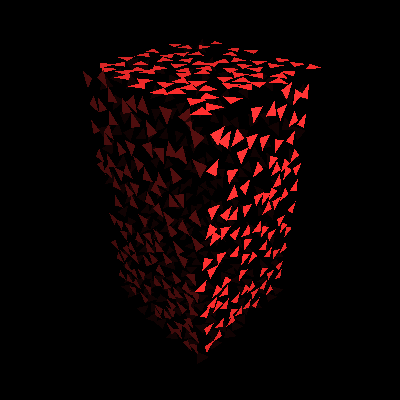
\includegraphics[width=50mm]{../img/box_1000_initial_points_quarter_size_430ms.png}}
   \\
   \subfloat[2000 points (5s 955ms)]{\label{fig:box2000s}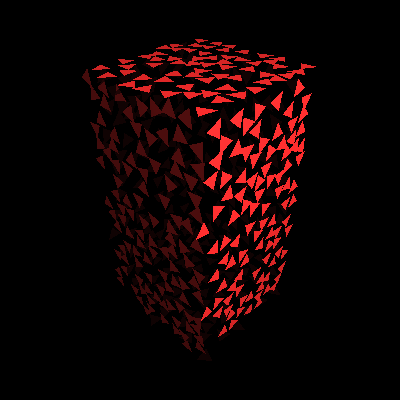
\includegraphics[width=50mm]{../img/box_2000_initial_points_quarter_size_5s955ms.png}}
   ~
   \subfloat[4000 points (43s 88ms)]{\label{fig:box4000s}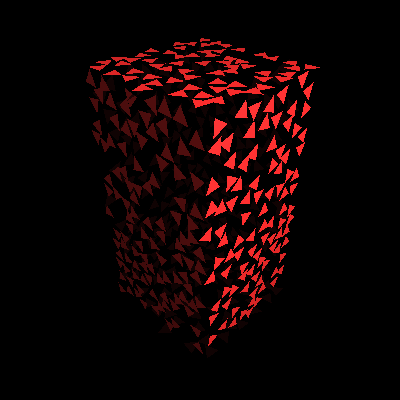
\includegraphics[width=50mm]{../img/box_4000_initial_points_quarter_size_43s88ms.png}}
   \\
   \subfloat[8000 points (6m 24s 803ms)]{\label{fig:box8000s}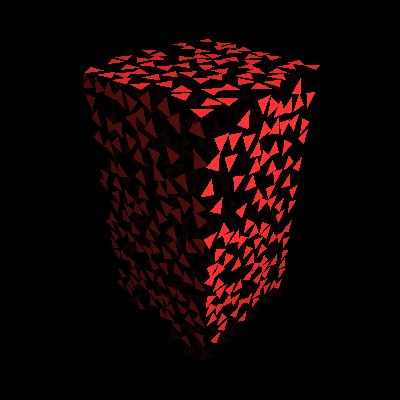
\includegraphics[width=50mm]{../img/box_8000_initial_points_quarter_size_6m24s803ms.png}}
   \captionfonts
   \caption[Box surfels at quarter size]{Surfel generation for a box, scaled in the y-axis, varying from 500 to 8000 initial points at quarter size. Generation times included in parenthesis.}
   \label{fig:small_box_surfels}
\end{figure}

\begin{figure}[h!]
   \centering
   \subfloat[500 points (1ms)]{\label{fig:box500}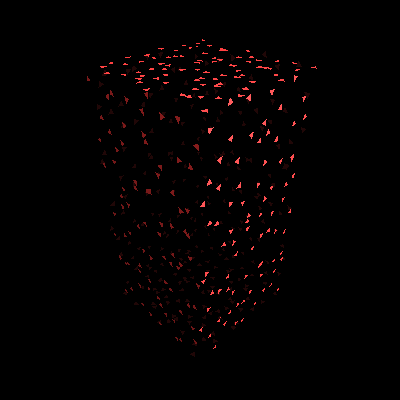
\includegraphics[width=50mm]{../img/box_500_initial_points_full_size_1ms.png}}
   ~
   \subfloat[1000 points (430ms)]{\label{fig:box1000}
\includegraphics[width=50mm]{../img/box_1000_initial_points_full_size_430ms.png}}
   \\
   \subfloat[2000 points (5s 927ms)]{\label{fig:box2000}
\includegraphics[width=50mm]{../img/box_2000_initial_points_full_size_5s927ms.png}}
   ~
   \subfloat[4000 points (43s 104ms)]{\label{fig:box4000}
\includegraphics[width=50mm]{../img/box_4000_initial_points_full_size_43s104ms.png}}
   \\
   \subfloat[8000 points (6m 24s 819ms)]{\label{fig:box8000}
\includegraphics[width=50mm]{../img/box_8000_initial_points_full_size_6m24s819ms.png}}
   \captionfonts
   \caption[Box surfels at full size]{Surfel generation for a box, scaled in the y-axis, varying from 500 to 8000 initial points at full size. Generation times included in parenthesis.}
   \label{fig:box_surfels}
\end{figure}

\begin{figure}[h!]
   \centering
   \subfloat[500 points (1ms)]{\label{fig:sphere500s}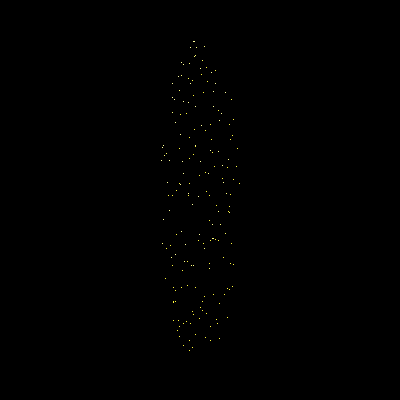
\includegraphics[width=50mm]{../img/sphere_500_initial_points_quarter_size_1ms.png}}
   ~
   \subfloat[1000 points (708ms)]{\label{fig:sphere1000s}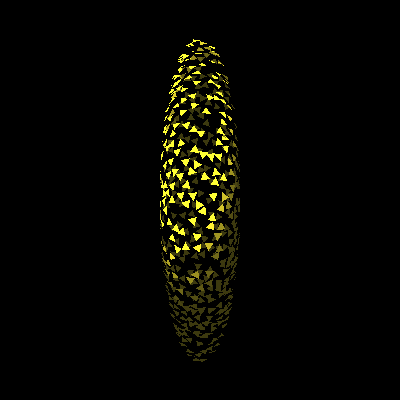
\includegraphics[width=50mm]{../img/sphere_1000_initial_points_quarter_size_708ms.png}}
   \\
   \subfloat[2000 points (6s 268ms)]{\label{fig:sphere2000s}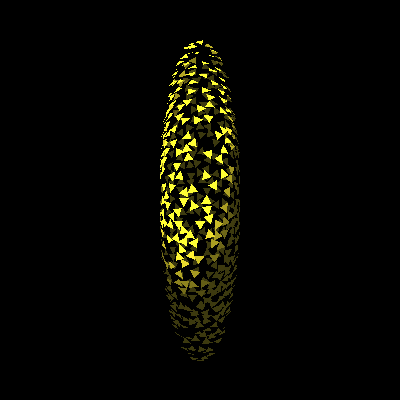
\includegraphics[width=50mm]{../img/sphere_2000_initial_points_quarter_size_6s268ms.png}}
   ~
   \subfloat[4000 points (51s 689ms)]{\label{fig:sphere4000s}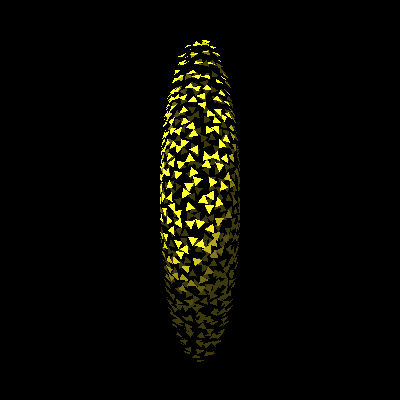
\includegraphics[width=50mm]{../img/sphere_4000_initial_points_quarter_size_51s689ms.png}}
   \\
   \subfloat[8000 points (6m 49s 391ms)]{\label{fig:sphere8000s}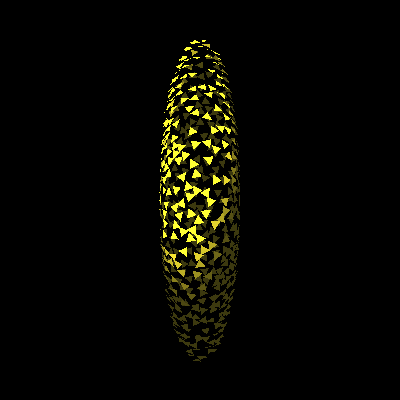
\includegraphics[width=50mm]{../img/sphere_8000_initial_points_quarter_size_6m49s391ms.png}}
   \captionfonts
   \caption[Sphere surfels at quarter size]{Surfel generation for a sphere, scaled in the y-axis, varying from 500 to 8000 initial points at quarter size. Generation times included in parenthesis.}
   \label{fig:small_sphere_surfels}
\end{figure}

\begin{figure}[h!]
   \centering
   \subfloat[500 points (1ms)]{\label{fig:sphere500}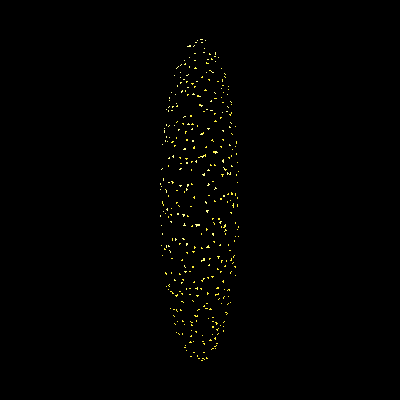
\includegraphics[width=50mm]{../img/sphere_500_initial_points_full_size_1ms.png}}
   ~
   \subfloat[1000 points (714ms)]{\label{fig:sphere1000}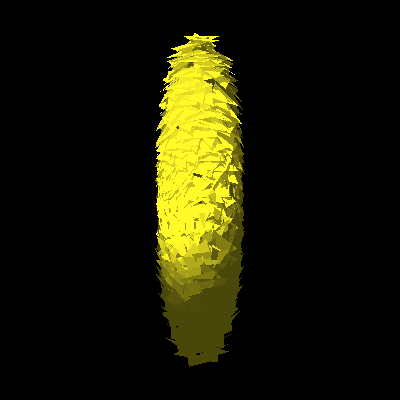
\includegraphics[width=50mm]{../img/sphere_1000_initial_points_full_size_714ms.png}}
   \\
   \subfloat[2000 points (6s 274ms)]{\label{fig:sphere2000}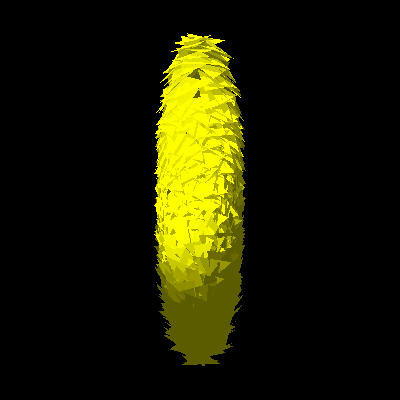
\includegraphics[width=50mm]{../img/sphere_2000_initial_points_full_size_6s274ms.png}}
   ~
   \subfloat[4000 points (51s 286ms)]{\label{fig:sphere4000}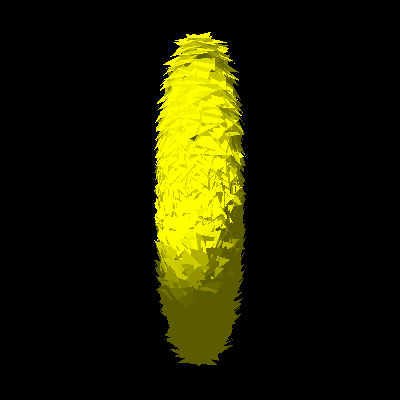
\includegraphics[width=50mm]{../img/sphere_4000_initial_points_full_size_51s286ms.png}}
   \\
   \subfloat[8000 points (6m 50s 309ms)]{\label{fig:sphere8000}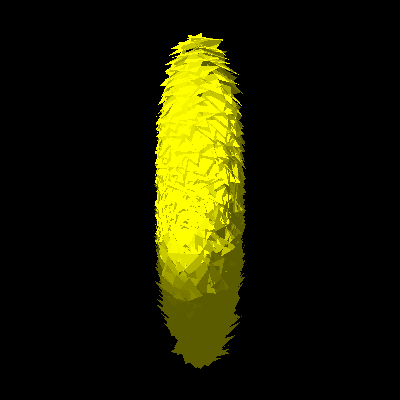
\includegraphics[width=50mm]{../img/sphere_8000_initial_points_full_size_6m50s309ms.png}}
   \captionfonts
   \caption[Sphere surfels at full size]{Surfel generation for a sphere, scaled in the y-axis, varying from 500 to 8000 initial points at full size. Generation times included in parenthesis.}
   \label{fig:sphere_surfels}
\end{figure}

\begin{figure}[h!]
   \centering
   \subfloat[500 points (1ms)]{\label{fig:tri500s}
\includegraphics[width=50mm]{../img/triangle_500_initial_point_5xMinDist_1ms.png}}
   ~
   \subfloat[1000 points (703ms)]{\label{fig:tri1000s}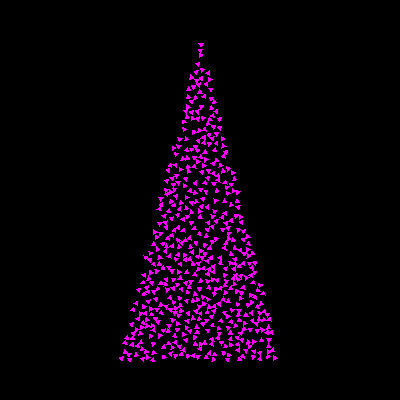
\includegraphics[width=50mm]{../img/triangle_1000_initial_point_5xMinDist_703ms.png}}
   \\
   \subfloat[2000 points (6s 283ms)]{\label{fig:tri2000s}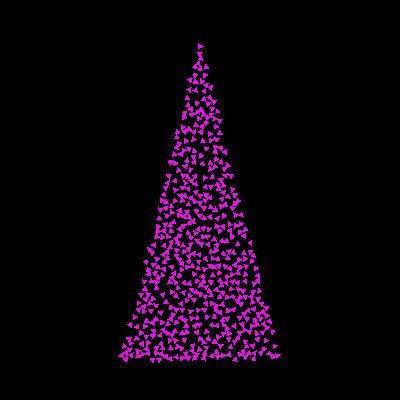
\includegraphics[width=50mm]{../img/triangle_2000_initial_point_5xMinDist_6s283ms.png}}
   ~
   \subfloat[4000 points (51s 432ms)]{\label{fig:tri4000s}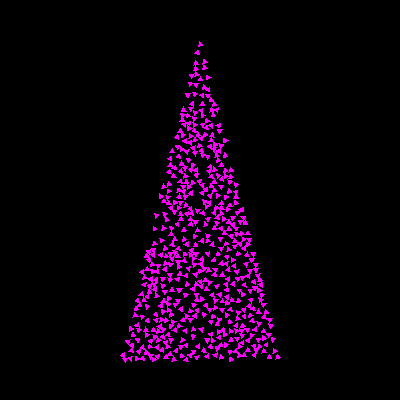
\includegraphics[width=50mm]{../img/triangle_4000_initial_point_5xMinDist_51s432ms.png}}
   \\
   \subfloat[8000 points (6m 49s 630ms)]{\label{fig:tri8000s}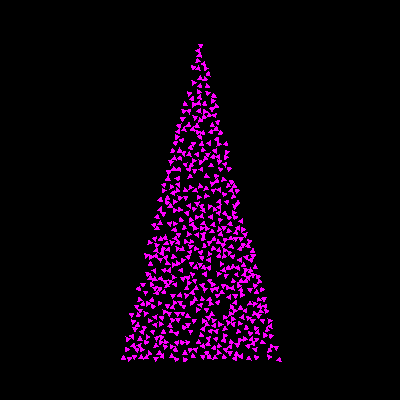
\includegraphics[width=50mm]{../img/triangle_8000_initial_point_5xMinDist_6m49s630ms.png}}
   \captionfonts
   \caption[Triangle surfels at quarter size]{Surfel generation for a triangle, scaled in the y-axis, varying from 500 to 8000 initial points at 1/4 size. Generation times included in parenthesis.}
   \label{fig:small_triangle_surfels}
\end{figure}

\begin{figure}[h!]
   \centering
   \subfloat[500 points (1ms)]{\label{fig:tri500}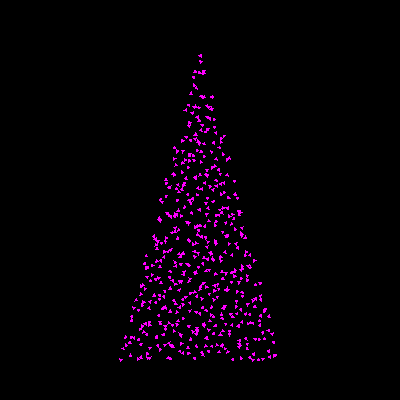
\includegraphics[width=50mm]{../img/triangle_500_initial_point_2xMinDist_1ms.png}}
   ~
   \subfloat[1000 points (713ms)]{\label{fig:tri1000}
\includegraphics[width=50mm]{../img/triangle_1000_initial_point_2xMinDist_713ms.png}}
   \\
   \subfloat[2000 points (6s 341ms)]{\label{fig:tri2000}
\includegraphics[width=50mm]{../img/triangle_2000_initial_point_2xMinDist_6s341ms.png}}
   ~
   \subfloat[4000 points (51s 279ms)]{\label{fig:tri4000}
\includegraphics[width=50mm]{../img/triangle_4000_initial_point_2xMinDist_51s279ms.png}}
   \\
   \subfloat[8000 points (6m 49s 847ms)]{\label{fig:tri8000}
\includegraphics[width=50mm]{../img/triangle_8000_initial_point_2xMinDist_6m49s847ms.png}}
   \captionfonts
   \caption[Triangle surfels at full size]{Surfel generation for a triangle, scaled in the y-axis, varying from 500 to 8000 initial points at full size. Generation times included in parenthesis.}
   \label{fig:triangle_surfels}
\end{figure}

% ---- SUBSECTION: VBO Storage ----
\subsection{VBO Storage}
\label{sec:VBOStorage}

The surfels are generated on the CPU, but they must be rendered by the GPU. Therefore, it is logical to store them in GPU memory. This avoids the latency of transferring data over the CPU-to-GPU bus, which we discuss in Section \ref{sec:cpu_v_gpu}. For this purpose we leverage the OpenGL Vertex Buffer Object, or VBO. This data structure is an array of vertices paired with colors. Additionally, we never update the surfel vertex data, so we can store them on the GPU during our pre-process.

%-------------------------------------------------------------------------------
% SECTION: Rendering
%-------------------------------------------------------------------------------
\section{Rendering}
\label{sec:rendering}
Our rendering algorithm follows standard ray-tracing as discussed in Section \ref{sec:ray_tracing_intro}, with the exception of the indirect lighting computation. The pseudocode is listed in Algorithm \ref{alg:gpu_pbcb}.

The indirect lighting computation uses our GPU PBCB algorithm and is the focus of this thesis. We describe the algorithm in detail in Section \ref{sec:indirect}, discuss the performance characteristics in Section \ref{ch:results}, analyze our results in Section \ref{sec:analysis}, and discuss future work in Section \ref{sec:future_work}.

% ---- SUBSECTION: Ray-Tracing ----
\subsection{Ray-Tracing}
\label{sec:rendering_ray_tracing}
Our ray-tracing algorithm follows the standards set in publications such as Peter Shirley's 'Fundamentals of Computer Graphics' \cite{bib:shirley_fundamentals}. First, we generate a list of rays, one per pixel, by iterating over all final-image pixels. As input we require a virtual camera definition, which provides a world-space location and field of view characteristics such as width and height of the final image. A ray is composed of an origin point, inherited from the virtual camera's location, and direction, calculated as the vector between the origin and associated pixel's center.

We then iterate over the list of rays, tracing them against the scene geometry to calculate their intersection point. The intersection algorithms are based on concepts from \cite{bib:pbr}, and \cite{verth:2008}.

Once we solve for the ray's intersection point with a geometric object, we calculate lighting. Because light calculations are additive \cite{bib:pbr}, we can split the calculation into a direct and an indirect computation.

Our direct lighting calculation is quite simple: in the case of point lighting, we simply trace one shadow ray \cite{bib:pbr} and if the path to the light is unobstructed, then we calculate standard Phong shading (see section \ref{sec:phong_model}), and in the case of area lighting we trace multiple shadow rays, in a uniform random distribution over the area light geometry, and scale the shading by the percent of unobstructed rays.

% ---- SUBSECTION: Anti-aliasing ----
%\subsection{Anti-aliasing}
%\label{sec:anti-aliasing}
%
%\begin{table}[h!]
%   \centering
%   \begin{tabular}{ | l | l | }
%   \hline
%   \textbf{AA Levels} & \textbf{Render Times} \\ \hline
%   1x1 (0x) & 103ms \\ \hline
%   2x2 (4x) & 382ms\\ \hline
%   3x3 (9x) & 843ms \\ \hline
%   4x4 (16x) & 1s 486ms \\ \hline
%   5x5 (25x) & 2s 302ms \\ \hline
%   \end{tabular}
%   \captionfonts
%   \caption[Anti-alias render times]{Render times for multiple levels of box filter anti-aliasing on our simple Cornell Box without indirect illumination.}
%   \label{tbl:aa_times}
%\end{table}

% ---- SUBSECTION: Indirect Gather via Rasterization (GPU PBCB) ----
\subsection{Indirect Gather via Rasterization (GPU PBCB)}
\label{sec:indirect}
By using the GPU's ability to rasterize triangles, we capture the incoming radiance at a ray intersection point by rasterizing our surfel cloud onto five 8 by 8 pixel textures arranged into a cube about the point. The cube represents the hemisphere used in the radiance integral (section \ref{sec:radiance}) . Using this technique, we attempt to realize a speedup over Monte Carlo ray-tracing as well as software-based PBCB. The psuedocode is listed in Algorithm \ref{alg:indirect_illum}.

\begin{algorithm}
\captionfont
\caption[Indirect Illumination]{Psuedocode for our Indirect Illumination algorithm.}
\label{alg:indirect_illum}
{\fontsize{10}{9}\selectfont
\begin{algorithmic}
   \Function{IndirectIllumination}{$intersection, scene$}
      \State $tangent$ := GramSchmidtTangent($intersection$.normal) //see alg. \ref{alg:unit_world_xform}
      \For{$i := 0...5$}
         \State $camera$ := ConstructCamera($i$, $intersection$.point, $intersection$.normal, $tangent$)
         \State $pixelData$ := Rasterize($camera$)
         \For{$j := 0...64$}
            \State $x := j$ \% $8$
            \State $y := j$ / $8$
            \State $right := -(camera.$up$ \times camera.$direction$)$
            \State $textureCenter := camera.$location$ + (nearPlane * camera.$direction$)$
            \State $a := -(7/8)$
            \State $b := 1/4$
            \State //see fig. \ref{fig:cubemap_texture}
            \State $jPixelCenter := textureCenter + (a*nearPlane + b*nearPlane*x)*right + (a*nearPlane + b*nearPlane*y)*camera.$up
            \State $sampleDirection$ := normalize($jPixelCenter - intersection.$point)
            \State $weight := intersection$.normal$ \cdot sampleDirection$
            \State $indirectColor$ += $weight * pixelData[j] * intersection$.surfaceColor
         \EndFor
      \EndFor
      \State $indirectColor$ /= $5 * 64$
      \State \Return $indirectColor$
   \EndFunction
\end{algorithmic}
}
\end{algorithm}

Our implementation utilizes the OpenGL API, along with helper libraries: GLUT and GLEW. Therefore, as a preamble to the algorithm, we must initialize OpenGL. This requires creating the OpenGL rendering context and associated buffers, and setting some constant state. In our case, we require an 8 by 8 pixel color texture and depth texture, and a vertex buffer with which we store our surfel data. Lastly, we set the constant rendering state by disabling OpenGL lighting such that the color we calculate in the surfel generation preprocess will be used directly, and by binding our textures and buffers, which informs OpenGL on how to use each buffer (e.g. render to color texture, or where vertex, color, and surface normal data is per triangle in the VBO).

As discussed in Section \ref{sec:rendering_ray_tracing} and \ref{sec:ray_tracing_intro}, the geometry intersection for each ray is computed, and then lighting for that point is calculated. And because light is linear \cite{bib:pbr}, we can calculate our indirect illumination separately from direct, and combine at a later time.

We begin our indirect illumination calculation for each intersection point by constructing five cameras that hold the render state required to rasterize each cube face. The cameras store their location, direction, up-vector, field of view, and near and far planes. The location for each camera is inherited from the intersection point. The direction is the intersection point's surface normal for the camera representing the top of the cube, and for the remaining cameras, we use the surface tangent, rotated in 90$^\circ$ increments. The up-vector for the cube-side cameras is the surface normal, and the top camera uses one of the side camera's direction vector. The field of view is set to 90$^\circ$ for each camera such that their viewing frustums fit together with no gaps (see figures \ref{fig:cubemap_top} \& \ref{fig:cubemap_side}). The near plane is set to 0.01, and the far plane is set to 15, which we have found offers good results for our test scene.

\begin{figure}[h!]
   \centering
   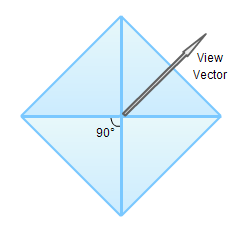
\includegraphics[width=100mm]{../img/cubemap_topview.png}
   \captionfonts
   \caption[Cubemap top-view]{Top view of the cameras that comprise our cube map.}
   \label{fig:cubemap_top}
\end{figure}

\begin{figure}[h!]
   \centering
   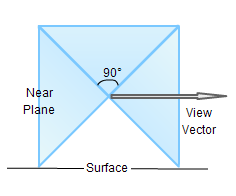
\includegraphics[width=100mm]{../img/cubemap_sideview.png}
   \captionfonts
   \caption[Cubemap side-view]{Side view of the cameras that comprise our cube map.}
   \label{fig:cubemap_side}
\end{figure}

Once the cube-face cameras are constructed, we iterate over each, and rasterize the surfel cloud onto an 8 by 8 pixel texture at the camera's near plane (see figure \ref{fig:cubemap_texture}). This texture data must then be read back from the GPU, and convolved into one indirect illumination value. We do this by iterating over each pixel, and adding it's contribution, calculated using the diffuse component of the Phong reflectance model (see section \ref{sec:phong_model}) to the final color.

\begin{figure}[h!]
   \centering
   \includegraphics[width=100mm]{../img/jPixelCenter.png}
   \captionfonts
   \caption[Cubemap texture]{View of the texture that is rasterized at the near plane of the camera.}
   \label{fig:cubemap_texture}
\end{figure}

Once each cube face has been rasterized and convolved, we return the final color as our indirect illumination value at the intersection point.

% ---- SUBSECTION: Final Color Computation ----
\subsection{Final Color Computation}

With the direct illumination calculated using the typical Phong shading technique \cite{bib:phong_thesis}, and the indirect illumination calculated via our algorithm, the final color is computed by adding the resultant values. This can be done because of the fact that light is linear \cite{bib:pbr}.

We then write the final color value to our image in memory. We store the final image in RAM until the rendering is complete, then write it to disk as an uncompressed TARGA image file.

%-------------------------------------------------------------------------------
% SECTION: Review
%-------------------------------------------------------------------------------
\section{Review}
We have presented a rendering algorithm that achieves an order of magnitude speedup over Monte Carlo ray-tracing on certain hardware, namely heterogenous chip architectures, with the knowledge that the future work discussed in Section \ref{sec:future_work} would extend our results to all hardware.

As an integral step of the algorithm, we have discussed our novel surfel generation algorithms for each of our supported primitives. Our surfel generation algorithms not only generate the triangles required by GPU-hardware for rasterization, but produce reasonably uniform coverage for arbitrarily transformed geometry.

Lastly, we discussed our indirect illumination computation: how we store our surfel cloud in GPU memory, rasterize it on to cube-map faces, and finally, convolve the cube-map pixels into one final color.

\endgroup

%---- Results and Discussion ----
\begingroup
\chapter{Results and Discussion}

%-------------------------------------------------------------------------------
% SECTION: Test Environment
%-------------------------------------------------------------------------------
\section{Test Environment}
Our test results were gathered on a 2011 MacBook Air [TODO]: 1.8Ghz Intel Core i7 (Sandy Bridge i7-2677M) [TODO], 4 GB 1333 MHz DDR3 SDRAM, Intel HD 3000 Graphics (on CPU-die) with 384 MB VRAM, and a solid-state (flash) hard disk.

%-------------------------------------------------------------------------------
% SECTION: Test Scene
%-------------------------------------------------------------------------------
\section{Test Scene}
Our test scene is an adapted Cornell Box. The Cornell Box was originally developed to quantify the difference between a Cornell renderer [TODO] and a real photograph of the same scene. However, due to its simple and elegant design, it has been adopted by the field of computer graphics as a standard for Global Illumination comparison (see [TODO], [TODO], [TODO]). Since its popularization circa TODO, it has become iconic and ubiquitous within the world of computer graphics. Originally, the Cornell Box contained just two cubes (as mimicked in our test scene), but the Cornell Box has been filled with many entities, such as: the Stanford Bunny [TODO], a chocolate-covered Stanford Bunny [TODO], multiple Stanford Bunnies [TODO], and a cow [TODO].

This scene was chosen for its ability to showcase the subtleties of indirect illumination. The overhead area light casts clearly visible soft shadows around the cubes, and the color bleeding from the walls of the Cornell Box is prominently displayed in those shadows. Another demonstrative feature is that no direct light is cast on the ceiling; it is illuminated by purely indirect light.

Our Cornell Box is defined in a modified POVRAY format [TODO], developed for the CSC 473 course at California Polytechnic State University, San Luis Obispo. It is comprised of 16 triangles, which make up the Cornell box, and 2 rotated and scaled cubes. This results in 14,000 surfels, following the algorithm in Section [TODO].

%-------------------------------------------------------------------------------
% SECTION: Analysis
%-------------------------------------------------------------------------------
\section{Analysis}

% ---- SUBSECTION: Memory ----
\subsection{Memory}
How much memory does the surfel cloud take up? ~1MB!

% ---- SUBSECTION: Speed ----
\subsection{Speed}

% ---- SUBSECTION: Image Quality ----
\subsection{Image Quality}
Check Chris' thesis for Perception based difference calculations.

% ---- SUBSECTION: Scalability ----
\subsection{Scalability}
Good for reasons specified in \cite{bib:christensen2008}. Discuss GPU memory for VBO though.

%-------------------------------------------------------------------------------
% SECTION: Conclusions
%-------------------------------------------------------------------------------
\section{Conclusions}
Doing a thesis is not easy.

%-------------------------------------------------------------------------------
% SECTION: Future Work
%-------------------------------------------------------------------------------
\section{Future Work}

% ---- SUBSECTION: Persistent Surfel Storage ----
\subsection{Persistent Surfel Storage}
Currently, our algorithm stores the surfels in RAM, not a persistent file on the hard drive. This requires our renderer to re-generate the surfels for each render. One of the main benefits of PBCB in production is that it is possible for a scene to have surfels generated, persistently stored in a file, and loaded at render time to be reused. This amortizes the cost of the surfel generation process across all renders for the same scene.

In our renderer, the most effective way to implement persistent surfel storage would be to write the VBO array memory to a file as binary data, as opposed to storing it as text mesh-file format. In this way, a simple memory map operation would map the data directly into the VBO structure without any text parsing and processing whatsoever.

For our Cornell box scene, the surfel generation takes 3 minutes per render[TODO], which could be avoided with persistent surfel storage. And although the surfel generation is not included in our render runtime results, the feature would increase our overall render throughput.

% ---- SUBSECTION: Dynamic Surfel Surface Area Computation ----
\subsection{Dynamic Surfel Surface Area Computation}
Having a dynamic density for surfels would help to homogenize the surfel size throughout the scene. Our algorithm naively creates a user-provided number of surfels per geometric primitive: for triangles and spheres, exactly the specified number of surfels are generated, and for boxes, each face generates the specified number (i.e. specified value multiplied by six per box). This results in vaiable surfel sizes across the same geometric primitive at different scales. For example, the smaller triangles that compose the ceiling of our Cornell box, and the larger triangles that compose the walls, both generate 500 surfels. Because the primitives have different surface areas, the surfel density is variable, resulting in small surfels for the small triangles, and larger surfels for the large triangles.

Our proposed solution to this problem is to have a user-provided surfel density in the form of minimum distance. The current algorithm would be modified to continue decimating the random points until the specified minimum distance is met. Another way in which to achieve the same result, in perhaps a more intuitive manner, would be to have a user-provided surfel surface area. We would then solve for the minimum distance that would provide such a surface area, and use that, per the previously described algorithm modification.

Furthermore, it would behoove us to analyze the results of varying the surfel surface area on final render quality and speed, as well as surfel memory requirements. The tradeoffs to consider are that larger surface areas would result in fewer surfels, thus requiring less memory and reducing render times by requiring fewer triangle rasterizations. But smaller surfels would increase the sampling density of the scene's radiance information, resulting in more accurate indirect illumination values, and would decrease the surfel generation run-time by requiring fewer passes for the decimation step within our algorithm.

% ---- SUBSECTION: Rasterization Batching ----
\subsection{Rasterizaiton Batching}
\label{subsec:raster-batching}
Due to the latency of GPU-to-GPU communication, it is in our best interest to batch as much of this communication as possible. In our algorithm, we raster each cube-face serially. This means that each 8x8 cube-face texture is rasterized, then copied from GPU to CPU memory, and processed. Therefore, each cube requires 5 data transfers (recall that the bottom of the cube is ignored). The communication from GPU to CPU can be reduced however.

We can accomplish fewer transfers by packing multiple cube-face textures into one single texture per cube. In this way, we amortize the cost of one GPU-to-CPU transfer over 5 textures. The algorithm for this technique would require one additional render pass, in which the 5 cube-face textures are texture-mapped to 5 screen-aligned quadrilaterals. This creates a texture atlas per cube that requires only one GPU-to-CPU transfer and can be indexed appropriately to extract the data for each cube-face.

This idea could be taken further: to batch the entire set of cubes, or some subset, as available memory and texture size dictates. Potentially, one thread could perform the standard direct illumination calculations via ray-tracing, while another thread rasterizes the surfel cloud onto cube-face textures, but stores them into one texture atlas for the entire scene. This is a very appealing idea to us because it would achieve great parallelism, as the CPU and GPU would be simultaneously leveraged to perform rendering tasks.

% ---- SUBSECTION: Parallelization ----
\subsection{Parallelization}
We believe the benefits of parallelization are apparent and will not discuss them further here. Suffice it to say that our algorithm can easily benefit from a model that divides primary pixels between multiple threads of control. In fact, this is precisely how our Monte Carlo ray-tracer accomplishes its parallelization. 

However, our code relies on the GLUT library [TODO] to create and manipulate the OpenGL context. GLUT does not currently support mulithreaded applications. For this reason, although our implementation supports multithreaded rendering for Monte Carlo ray-tracing, it does not for our GPU Point-Based Color Bleeding algorithm. We have acquired our results in both cases with one thread only.
 
Any solution to this problem will involve porting the OpenGL code that leverages GLUT to another multithreading-friendly library. BLAH is one such library that is freely available [TODO]. Preferably, the library would support one single context that is shared between all threads of control and serializes their access. By sharing the context, the surfel data within the VBO memory does not need to be duplicated.

Another type of parallelization that many applications utilizing the GPU leverage is CPU-GPU parallelization. This is where concurrent work is performed on both hardware devices. That is to say: the CPU does not block on a GPU draw call. This can be accomplished via the process described in subsection \ref{subsec:raster-batching}. Here, we can completely divide the rendering process into threads performing direct illumination via standard ray-tracing and threads performing indirect illumination via GPU PBCB. Because our two types of illumination have no interdependencies, two final images can be rendered, one with the direct illumination values, and the other with the indirect illumination values, and combined after both rendering passes are complete.


\endgroup

%% ------------- End main chapters ----------------------

\clearpage
\bibliography{thesis}

\end{document}
